% !TEX TS-program = lualatex
% !TEX encoding = UTF-8 Unicode

\documentclass[12pt, letterpaper]{article}

%%BIBLIOGRAPHY- This uses biber/biblatex to generate bibliographies according to the 
%%Unified Style Sheet for Linguistics
\usepackage[main=american, german]{babel}% Recommended
\usepackage{csquotes}% Recommended
\usepackage[backend=biber,
             style=unified,
             maxcitenames=3,
             maxbibnames=99,
             natbib,
             url=false]{biblatex}
\addbibresource{Library.bib}
\setcounter{biburlnumpenalty}{100}  % allow URL breaks at numbers
%\setcounter{biburlucpenalty}{100}   % allow URL breaks at uppercase letters
%\setcounter{biburllcpenalty}{100}   % allow URL breaks at lowercase letters

%%TYPOLOGY
\usepackage[svgnames]{xcolor} % Specify colors by their 'svgnames', for a full list of all colors available see here: http://www.latextemplates.com/svgnames-colors
%\usepackage[compact]{titlesec}
%\titleformat{\section}[runin]{\normalfont\bfseries}{\thesection.}{.5em}{}[.]
%\titleformat{\subsection}[runin]{\normalfont\scshape}{\thesubsection}{.5em}{}[.]
\usepackage[hmargin=1in,vmargin=1in]{geometry}  %Margins
\usepackage{graphicx} % 
\usepackage{stackengine} %Package to allow text above or below other text, Also helpful for HG weights 
\usepackage{fontspec} %Selection of fonts must be ran in XeLaTeX
\usepackage{amssymb} %Math symbols
\usepackage{amsmath} % Mathematical enhancements for LaTeX
\usepackage{setspace} %Linespacing
\usepackage{multicol} %Multicolumn text
\usepackage{enumitem} %Allows for continuous numbering of lists over examples, etc.
\usepackage{multirow} %Useful for combining cells in tablesbrew 
\usepackage{booktabs}
\usepackage{hanging}
\usepackage{fancyhdr} %Allows for the 
\pagestyle{fancy}
\fancyhead[L]{\textit{QP Defense Handout}} 
\fancyhead[R]{\textit{\today}} 
\fancyfoot[L,R]{} 
\fancyfoot[C]{\thepage} 
\renewcommand{\headrulewidth}{0.4pt}
\setlength{\headheight}{14.5pt} % ...at least 14.49998pt
% \usepackage{fourier} % This allows for the use of certain wingdings like bombs, frowns, etc.
% \usepackage{fourier-orns} %More useful symbols like bombs and jolly-roger, mostly for OT
\usepackage[colorlinks,allcolors={black},urlcolor={blue}]{hyperref} %allows for hyperlinks and pdf bookmarks
% \usepackage{url} %allows for urls
% \def\UrlBreaks{\do\/\do-} %allows for urls to be broken up
\usepackage[normalem]{ulem} %strike out text. Handy for syntax
\usepackage{tcolorbox}
\usepackage{datetime2}
\usepackage{caption}
\usepackage{subcaption}

%%FONTS
\setmainfont{Libertinus Serif}
\setsansfont{Libertinus Sans}
\setmonofont[Scale=MatchLowercase]{Libertinus Mono}

%%PACKAGES FOR LINGUISTICS
%\usepackage{OTtablx} %Generating tableaux with using TIPA
\usepackage[noipa]{OTtablx} % Use this one generating tableaux without using TIPA
%\usepackage[notipa]{ot-tableau} % Another tableau drawing packing use for posters.
% \usepackage{linguex} % Linguistic examples
% \usepackage{langsci-linguex} % Linguistic examples
\usepackage{langsci-gb4e} % Language Science Press' modification of gb4e
% \usepackage{langsci-avm} % Language Science Press' AVM package
\usepackage{tikz} % Drawing Hasse diagrams
% \usepackage{pst-asr} % Drawing autosegmental features
\usepackage{pstricks} % required for pst-asr, OTtablx, pst-jtree.
% \usepackage{pst-jtree} %Syntax tree draawing software
% \usepackage{tikz-qtree} % Another syntax tree drawing software. Uses bracket notation.
\usepackage[linguistics]{forest} % Another syntax tree drawing software. Uses bracket notation.
% \usepackage{ling-macros} % Various linguistic macros. Does not work with linguex.
% \usepackage{covington} % Another linguistic examples package.
\usepackage{leipzig} % Offers support for Leipzig Glossing Rules

%%LEIPZIG GLOSSING FOR ZAPOTEC
\newleipzig{el}{el}{elder} % Elder pronouns
\newleipzig{hu}{hu}{human} % Human pronouns
\newleipzig{an}{an}{animate} % Animate pronouns
\newleipzig{in}{in}{inanimate} % Inanimate pronouns
\newleipzig{pot}{pot}{potential} % Potential Aspect
\newleipzig{cont}{cont}{continuative} % Continuative Aspect
% \newleipzig{pot}{pot}{potential} % Potential Aspect
\newleipzig{stat}{stat}{stative} % Potential Aspect
\newleipzig{and}{and}{andative} % Andative Aspect
\newleipzig{ven}{ven}{venative} % Venative Aspect
% \newleipzig{res}{res}{restitutive} % Restitutive Aspect
\newleipzig{rep}{rep}{repetitive} % Repetitive Aspect

%%TITLE INFORMATION
\title{TITLE}
\author{Mykel Loren Brinkerhoff}
\date{\today}

%%MACROS
\newcommand{\sub}[1]{\textsubscript{#1}}
\newcommand{\supr}[1]{\textsuperscript{#1}}
\providecommand{\lsptoprule}{\midrule\toprule}
\providecommand{\lspbottomrule}{\bottomrule\midrule}
\newcommand{\fittable}[1]{\resizebox{\textwidth}{!}{#1}}

\makeatletter
\renewcommand{\paragraph}{%
  \@startsection{paragraph}{4}%
  {\z@}{0ex \@plus 1ex \@minus .2ex}{-1em}%
  {\normalfont\normalsize\bfseries}%
}
\makeatother
\parindent=10pt


\begin{document}

%%If using linguex, need the following commands to get correct LSA style spacing
%% these have to be after  \begin{document}
    % \setlength{\Extopsep}{6pt}
    % \setlength{\Exlabelsep}{9pt}%effect of 0.4in indent from left text edge
%%

%% Line spacing setting. Comment out the line spacing you do not need. Comment out all if you want single spacing.
%\doublespacing
%\onehalfspacing

\begin{center}
    {\Large \textbf{The acoustics of phonation in Santiago Laxopa Zapotec}}\footnote{I am grateful to Fe Silva-Robles and  Raúl Díaz Robles for sharing their time and language expertise. I am also grateful to Grant McGuire,  Jaye Padgett, Rachel Walker, Maziar Toosarvandani, Ben Eischens, Kim Tan, and Zach Horton for their help and discussions during all stages of this project. This project branched off of a collaboration with Jack Duff and Maya Wax Cavallaro. Various parts of this project were previously shared in joint presentations with Jack Duff and Maya Wax Cavallaro.
	
	This work was supported in part by the National Science Foundation under Grant No. 2019804, the Humanities Institute at UC Santa Cruz, and the Jacobs Research Funds.}
    \vspace{6pt}

    Mykel Loren Brinkerhoff
\end{center}
%\maketitle
%\maketitleinst
\thispagestyle{fancy}

% \tableofcontents

%------------------------------------
\section{Introduction} \label{sec:Introduction}
%------------------------------------

\begin{itemize}
    \item Phonation is a process where the larynx is used to alter the way different sounds are produced. 
	\item This use of the larynx produces sounds which vary from being more breathy or creaky.
	\begin{itemize}
		\item Other types of phonation also exist (see \cite{eslingVoiceQualityLaryngeal2019} for a detailed discussion on the different phonation types that exist and how the larynx produces them).
	\end{itemize} 
	\item In some languages these alterations are described as being pathological, with some speakers just being more breathy or creaky than others (e.g., \cite{klattAnalysisSynthesisPerception1990}). 
    \item In other languages these phonation types are used phonemically like in Gujarati, where vowels can be breathy or modal \citep{fischer-jorgensenPhoneticAnalysisBreathy1968}. 
    \item This phonemic use of phonation is particularly common in the Otomanguean language family from southern Mexico (e.g., \cite{suarezMesoamericanIndianLanguages1983,campbellMesoAmericaLinguisticArea1986,silvermanLaryngealComplexityOtomanguean1997,campbellOtomangueanHistoricalLinguistics2017a,campbellOtomangueanHistoricalLinguistics2017}).
    \item One of the common problems facing linguists who study phonation is determining what the acoustic correlates are for these different phonation types. 
    \item This paper is a preliminary investigation into the acoustic correlates of the different phonation types in Santiago Laxopa Zapotec, an Otomanguean language spoken by approximately 1200 people.
    \item I show that that H1-H2 is not a very good indicator of phonation in Santiago Laxopa Zapotec, but like other Zapotecs H1-A3 is a good indicator of phonation. 
    \item Additionally, Cepstral Peak Prominence is shown to be useful in distinguishing checked and laryngealized vowels apart for one of the speakers.
\end{itemize}

%------------------------------------
\section{Background} \label{sec:Background}
%------------------------------------

\begin{itemize}
	\item It is commonly assumed that the vocal folds, which account for differences in pitch and voicing, are also responsible for differences in phonation. 
	\item \citet{ladefogedPreliminariesLinguisticPhonetics1971,gordonPhonationTypesCrosslinguistic2001} argued that phonation exists on a single dimension ranging from opened vocal folds to closed vocal folds. 
	\item The variation in how open or closed the vocal folds are correspond to whether or not the sound produced is breathy or creaky. 
	\item \citet{ladefogedPreliminariesLinguisticPhonetics1971,gordonPhonationTypesCrosslinguistic2001} summarized this assumption in the diagram found in Figure~\ref{fig:Phonation}.
\end{itemize}

\begin{figure}[!h]
	\centering
	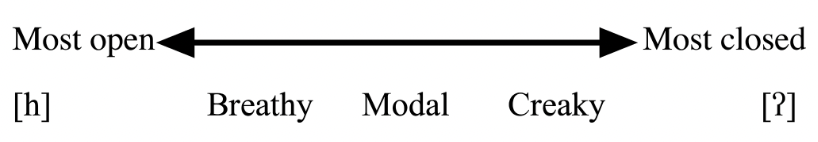
\includegraphics[width=.6\textwidth]{../Phonation.png}
	\caption{Simplified one-deminsional model for phonation. Based on \citet{ladefogedPreliminariesLinguisticPhonetics1971,gordonPhonationTypesCrosslinguistic2001}}.
	\label{fig:Phonation}
\end{figure}

\begin{itemize}
	\item In addition to this degree of openness, linguists have found that there are other acoustic measurements that correlate to different types of phonation. 
	\item Commonly, these acoustic measurements are spectral-tilt measurements. 
	\item Spectral-tilt measurements are when you take the relative amplitude of different harmonics and subtract them from each other. 
	\item \cite{fischer-jorgensenPhoneticAnalysisBreathy1968} showed that the difference between the amplitude of the first harmonic and second harmonic can account for the differences between breathy and modal vowels. 
\end{itemize}

\begin{figure}[!h]
	\centering
	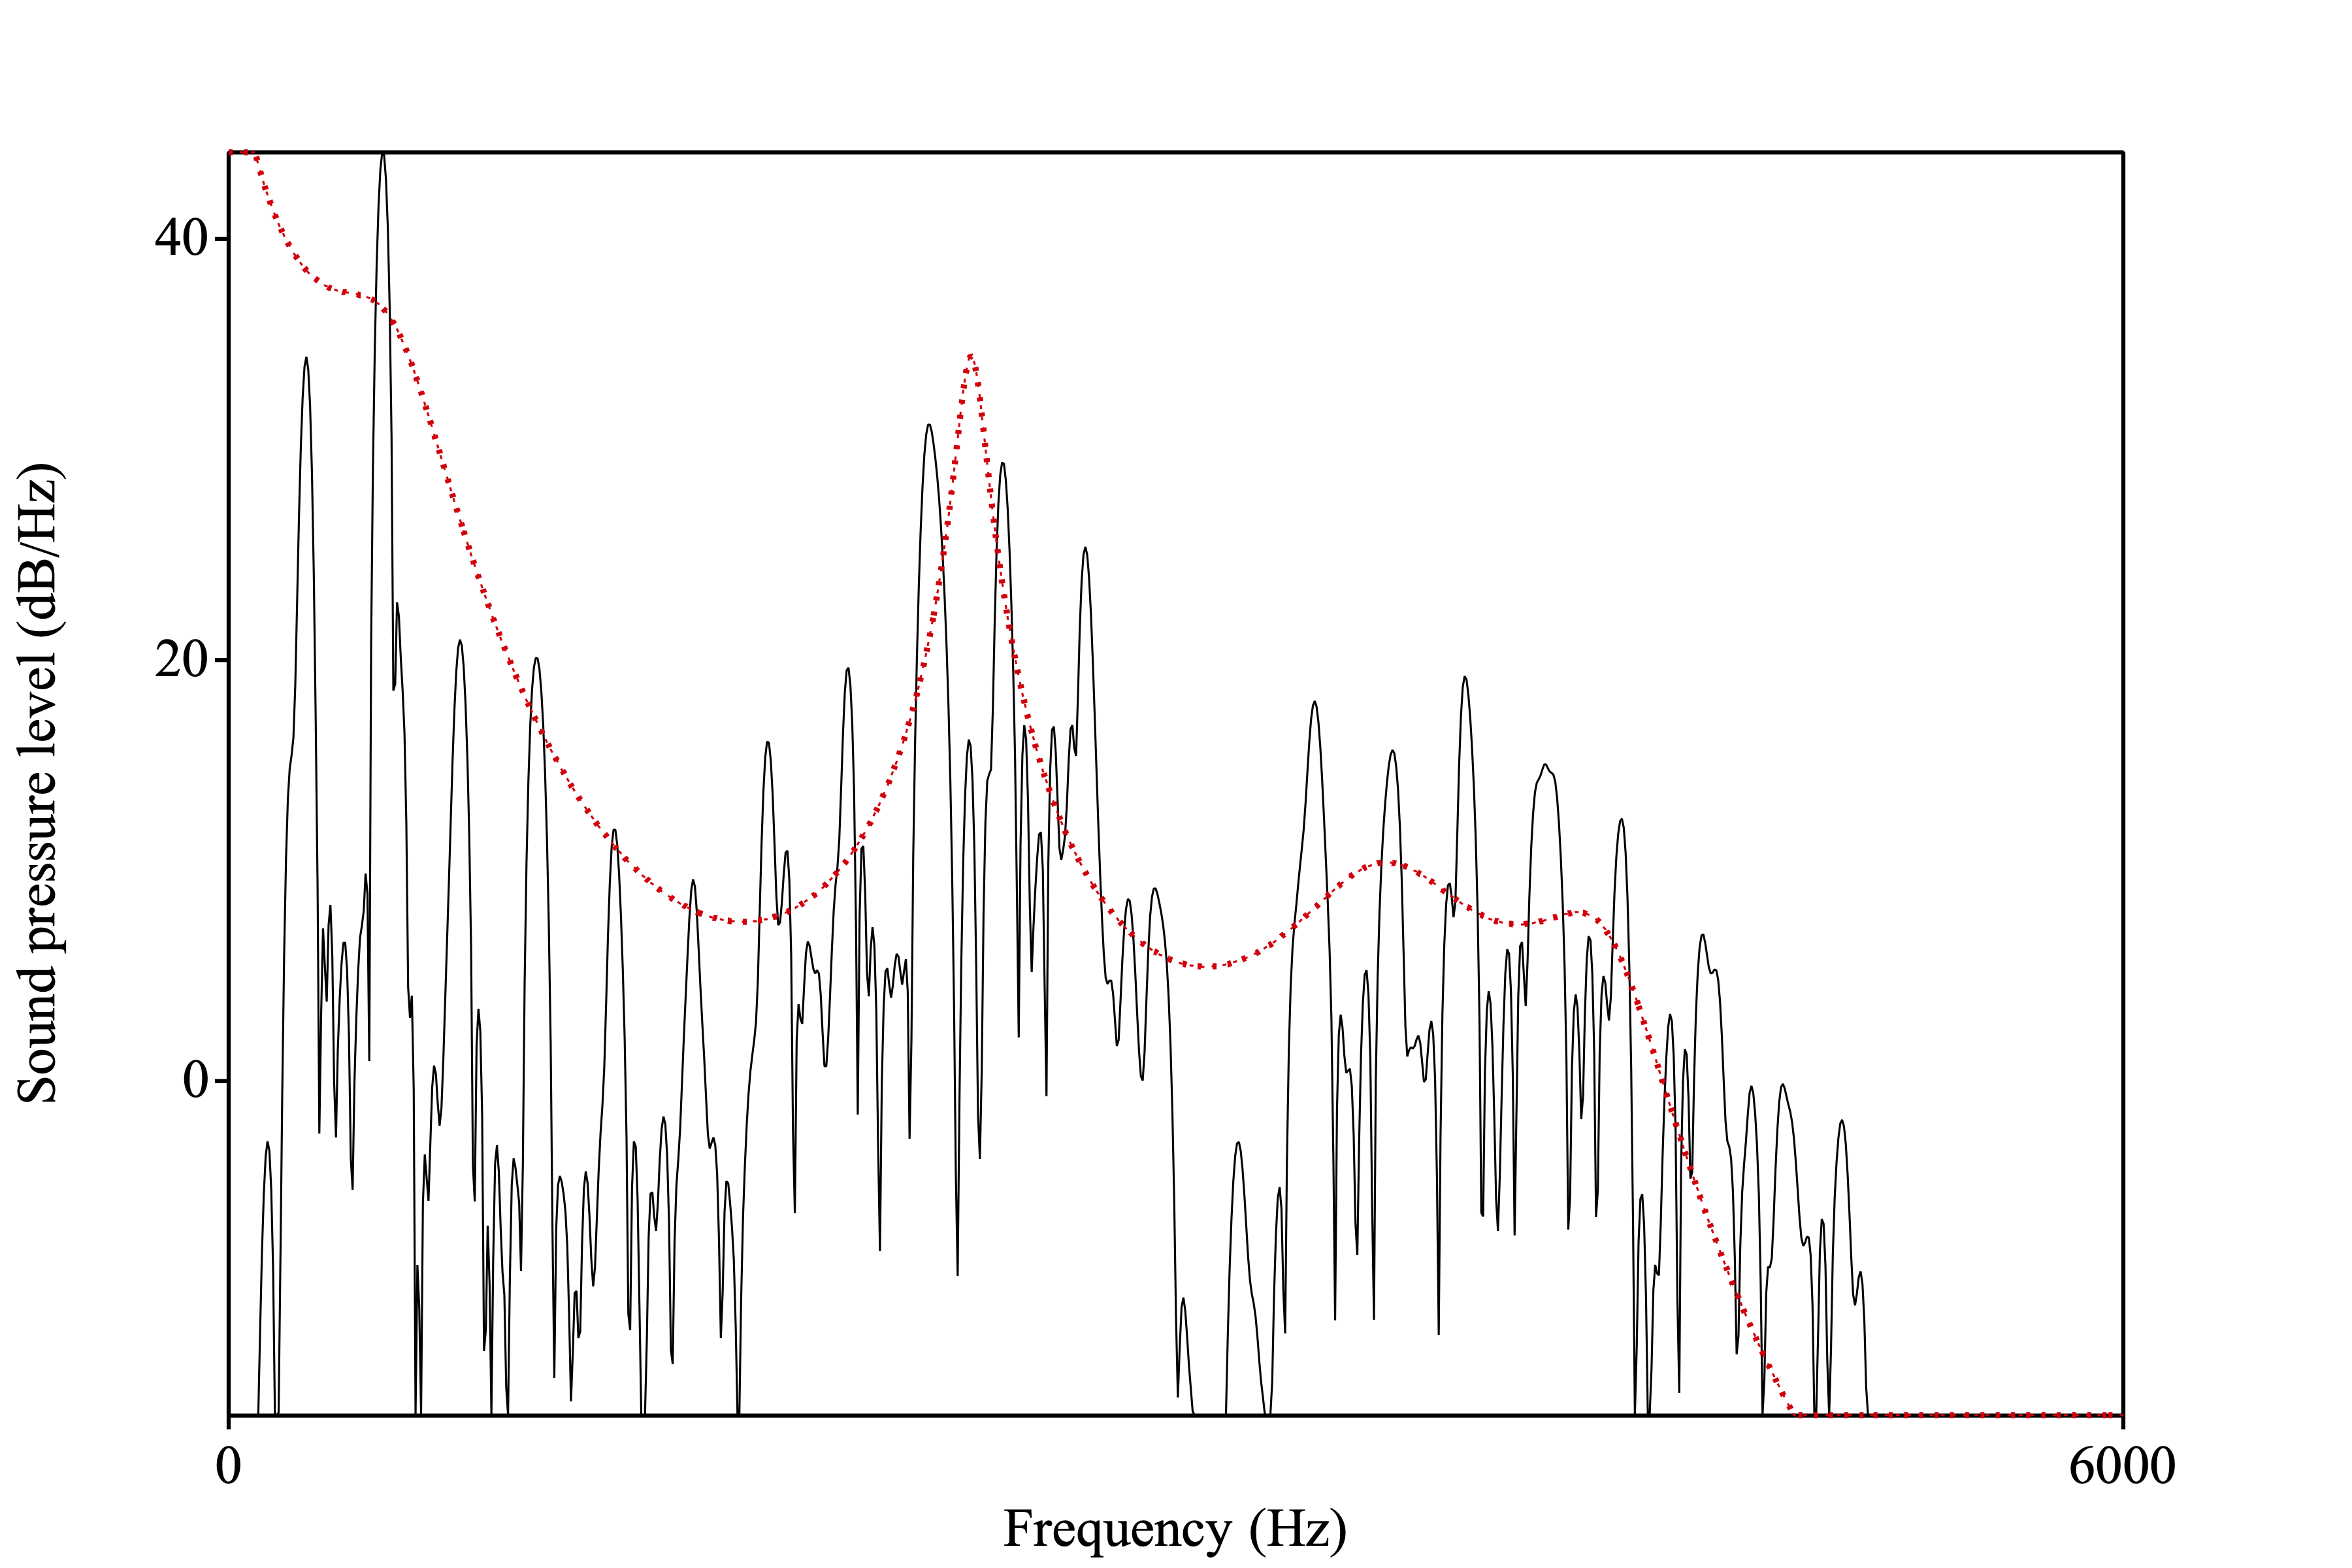
\includegraphics[width=0.9\textwidth]{../Harmonics.png}
	\caption{Spectral slice with LPC smoothed line overlaid for the vowel [e]. The harmonics in the spectral slice are represented by each of the dark peaks. The leftmost black solid line peak is the first harmonic (H1) and each subsequent peak represents the next highest harmonic (H2 through H\textit{n}). The red dotted line represents an LPC smoothed line which identifies the formants by the peaks. Each of the harmonics that are closest to the formant peak is identified as A1 through A\textit{n}.}
	\label{fig:Harmonics}
\end{figure}
%------------------------------------
\section{Santiago Laxopa Zapotec} \label{sec:SLZ}
%------------------------------------

\begin{itemize}
    \item Santiago Laxopa Zapotec (SLZ), endonym \textit{Dille'xhunh Laxup}, is a a Northern Zapotec language spoken by approximately 1000 people in the municipality of Santiago Laxopa, Ixtlán, Oaxaca, Mexico and in diaspora communities in Mexico and the United States \citep{adlerAcousticsPhonationTypes2016,adlerDerivationVerbInitiality2018,foleyForbiddenCliticClusters2018,foleyExtendingPersonCaseConstraint2020}.
    \item Closely related to San Bartolomé Zoogocho Zapotec \citep{longDiccionarioZapotecoSan2005,sonnenscheinDescriptiveGrammarSan2005} and shares a high level of mutual intelligibility with it.
    \item SLZ is similar to other Zapotecan languages in distinguishing lenis and fortis consonants \citep[e.g.,][]{nellisFortisLenisCajonos1980,jaegerFortisLenisQuestion1983,uchiharaFortisLenisGlides2016}.
\end{itemize}

\begin{table}[!h]
	\centering
	\caption{Consonant inventory for Santiago Laxopa Zapotec}
	\label{tab:SLZcons}
	\fittable{
	\begin{tabular}{llcccccccc}
	\lsptoprule
		  &  & bilabial & alveolar  & post- & retroflex & palatal &velar &labio-  &  uvular \\
		 &&&&alveolar&  &&&velar& \\
	\midrule
	stop 		& lenis   & b  & d  & & & & g & gʷ & \\
				& fortis  & p  & t  & & & & k & kʷ & \\
	fricative   & lenis   &    & z  & ʒ & ʐ &  & &  & ʁ \\
		        & fortis  &    & s  & ʃ & ʂ & ç & & & \\
	affricate 	& lenis   &    & d͡z & & & & & & \\
				& fortis  &    & t͡s & & t͡ʃ & & & & \\
    nasal    	& lenis   &	   & n  & & & & & & \\
				& fortis  &	mː & nː & & & & & & \\
	lateral  	& lenis   &    & l & & & & & & \\
				& fortis  &    & lː & & & & & & \\
	trill		& 		  &    & r & & &  & &  & \\ 			
	approximate & 		  &    & & & & & & w & \\ 
	\lspbottomrule
	\end{tabular}
	}
\end{table}

\begin{itemize}
    \item SLZ has a standard five vowel inventory. 
\end{itemize}

\begin{table}[!h]
	\centering
	\caption{Vowel qualities in Santiago Laxopa Zapotec.}
    \label{tab:SLZvowels}
	\begin{tabular}{lccc}
	\lsptoprule
	&  front& central  & back \\
	\midrule
	high   	&  i  &     &   u \\
	mid    	&  e  &   	& 	o \\
	low   	&     &  a 	&	  \\
	\lspbottomrule
	\end{tabular}
\end{table}

\begin{itemize}
	\item These five vowels, additionally, appear with one of four different phonation types which will be discussed in greater detail in Section~\ref{sec:Phonation}.
\end{itemize}

%------------------------------------
\subsection{Tone in Santiago Laxopa Zapotec} \label{sec:Tone}
%------------------------------------

\begin{itemize}
    \item Similar to other Otomanguean languages, SLZ is tonal \citep{suarezMesoamericanIndianLanguages1983,campbellMesoAmericaLinguisticArea1986,silvermanLaryngealComplexityOtomanguean1997,campbellOtomangueanHistoricalLinguistics2017a,campbellOtomangueanHistoricalLinguistics2017}.
    \item SLZ has five distinct tonal patterns that appear on the syllables of nouns, see Table~\ref{tab:tones}. 
\end{itemize}

\begin{table}[!h]
	\centering
	\caption{Examples of the five tonal patterns observed in the Santiago Laxopa Zapotec words.}
	\label{tab:tones}
	\begin{tabular}{lllll}
	\lsptoprule
	High   	&  a\supr{H}  &  \textit{xha}   &  [ ʐa\supr{H} ] & `clothing.\textsc{poss}'\\
	Mid    	&  a\supr{M}  &  \textit{lhill} 	& [ liʒ\supr{M} ] & `house.\textsc{poss}' \\
	Low   	&  a\supr{L}  &  \textit{yu'} 	&	 [ çuˀ\supr{L} ] & `earth'\\
	Rising	&  a\supr{MH}  &  \textit{yu'u} 	&	[ çuˀu\supr{MH} ] & `quicklime (Sp. cal)' \\
	Falling &  a\supr{HL}  &  \textit{yu'u}  &	[ çuˀu\supr{HL} ] &	`house' \\
	\lspbottomrule
	\end{tabular}
\end{table}

\begin{itemize}
	\item These five tonal patterns are illustrated in Figures~\ref{fig:FSRTonePlot} and \ref{fig:RDTonePlot} for two different SLZ speakers. 
	\item Figures~\ref{fig:FSRTonePlot} and \ref{fig:RDTonePlot} shows the five tonal contrasts averaged for each tonal contrast from the onset to ending of the vowel. 
	\item The first 20-25\% of Figures~\ref{fig:FSRTonePlot} and \ref{fig:RDTonePlot} can be ignored due to the influence of consonantal transitions. 
\end{itemize}

\begin{figure}[!ht]
	\centering
	\includegraphics[width=0.9\textwidth]{../FSRTonePlot.png}
	\caption{Tonal contrasts for FSR averaged and time normalized. Each line in this graph represents the average of approximately 10 syllables for each tonal pattern. }
	\label{fig:FSRTonePlot}
\end{figure}

\begin{figure}[!ht]
	\centering
	\includegraphics[width=0.9\textwidth]{../RDTonePlot.png}
	\caption{Tonal contrasts for RD averaged and time normalized. Each line in this graph represents the average of approximately 10 syllables for each tonal pattern.}
	\label{fig:RDTonePlot}
\end{figure}

\begin{itemize}
	\item Evidence from \citet{brinkerhoffDownstepSantiagoLaxopaMFM,brinkerhoffTonalPatternsTheir2022}, however, suggests that the five tonal patterns are epiphenomenal in SLZ.
	\begin{itemize}
		\item Similar to what \citet{mcphersonWordToneEpiphenomenal2022} found for Poko (Skou, PNG).
	\end{itemize}
\end{itemize}
%------------------------------------
\subsection{Phonation in Santiago Laxopa Zapotec} \label{sec:Phonation}
%------------------------------------

\begin{itemize}
	\item Zapotecan languages commonly make use of contrastive phonation on vowels \citep[e.g.,][]{avelinobecerraTopicsYalalagZapotec2004,longDiccionarioZapotecoSan2005,avelinoAcousticElectroglottographicAnalyses2010,lopeznicolasEstudiosFonologiaGramatica2016,chavez-peonInteractionMetricalStructure2010,ariza-garciaPhonationTypesTones2018}.
	\item SLZ has four contrastive phonation types: modal /a/, breathy /a̤/, checked /aˀ/, and laryngealized /aˀa/.
\end{itemize}

\ea \label{ex:YA} Four-way near minimal phonation contrast
	\ea \textit{yag}  [çag\supr{L}] `tree; wood; almúd (unit of measurement approximately 4kg)'
	\ex \textit{yah}  [ça̤\supr{L}] `metal; rifle; bell'
	\ex \textit{yu'}  [çuˀ\supr{L}]  `earth'
	\ex \textit{ya'a}  [çaˀa\supr{L}]  `market'
	\z 
\z 

\begin{itemize}
	\item Breathy phonation on vowels is characterized by a raspy quality throughout the whole vowel or a portion toward the end of the vowel, see Figure~\ref{fig:BreathyVowel}. 
\end{itemize}

\begin{figure}[!h]
	\centering
	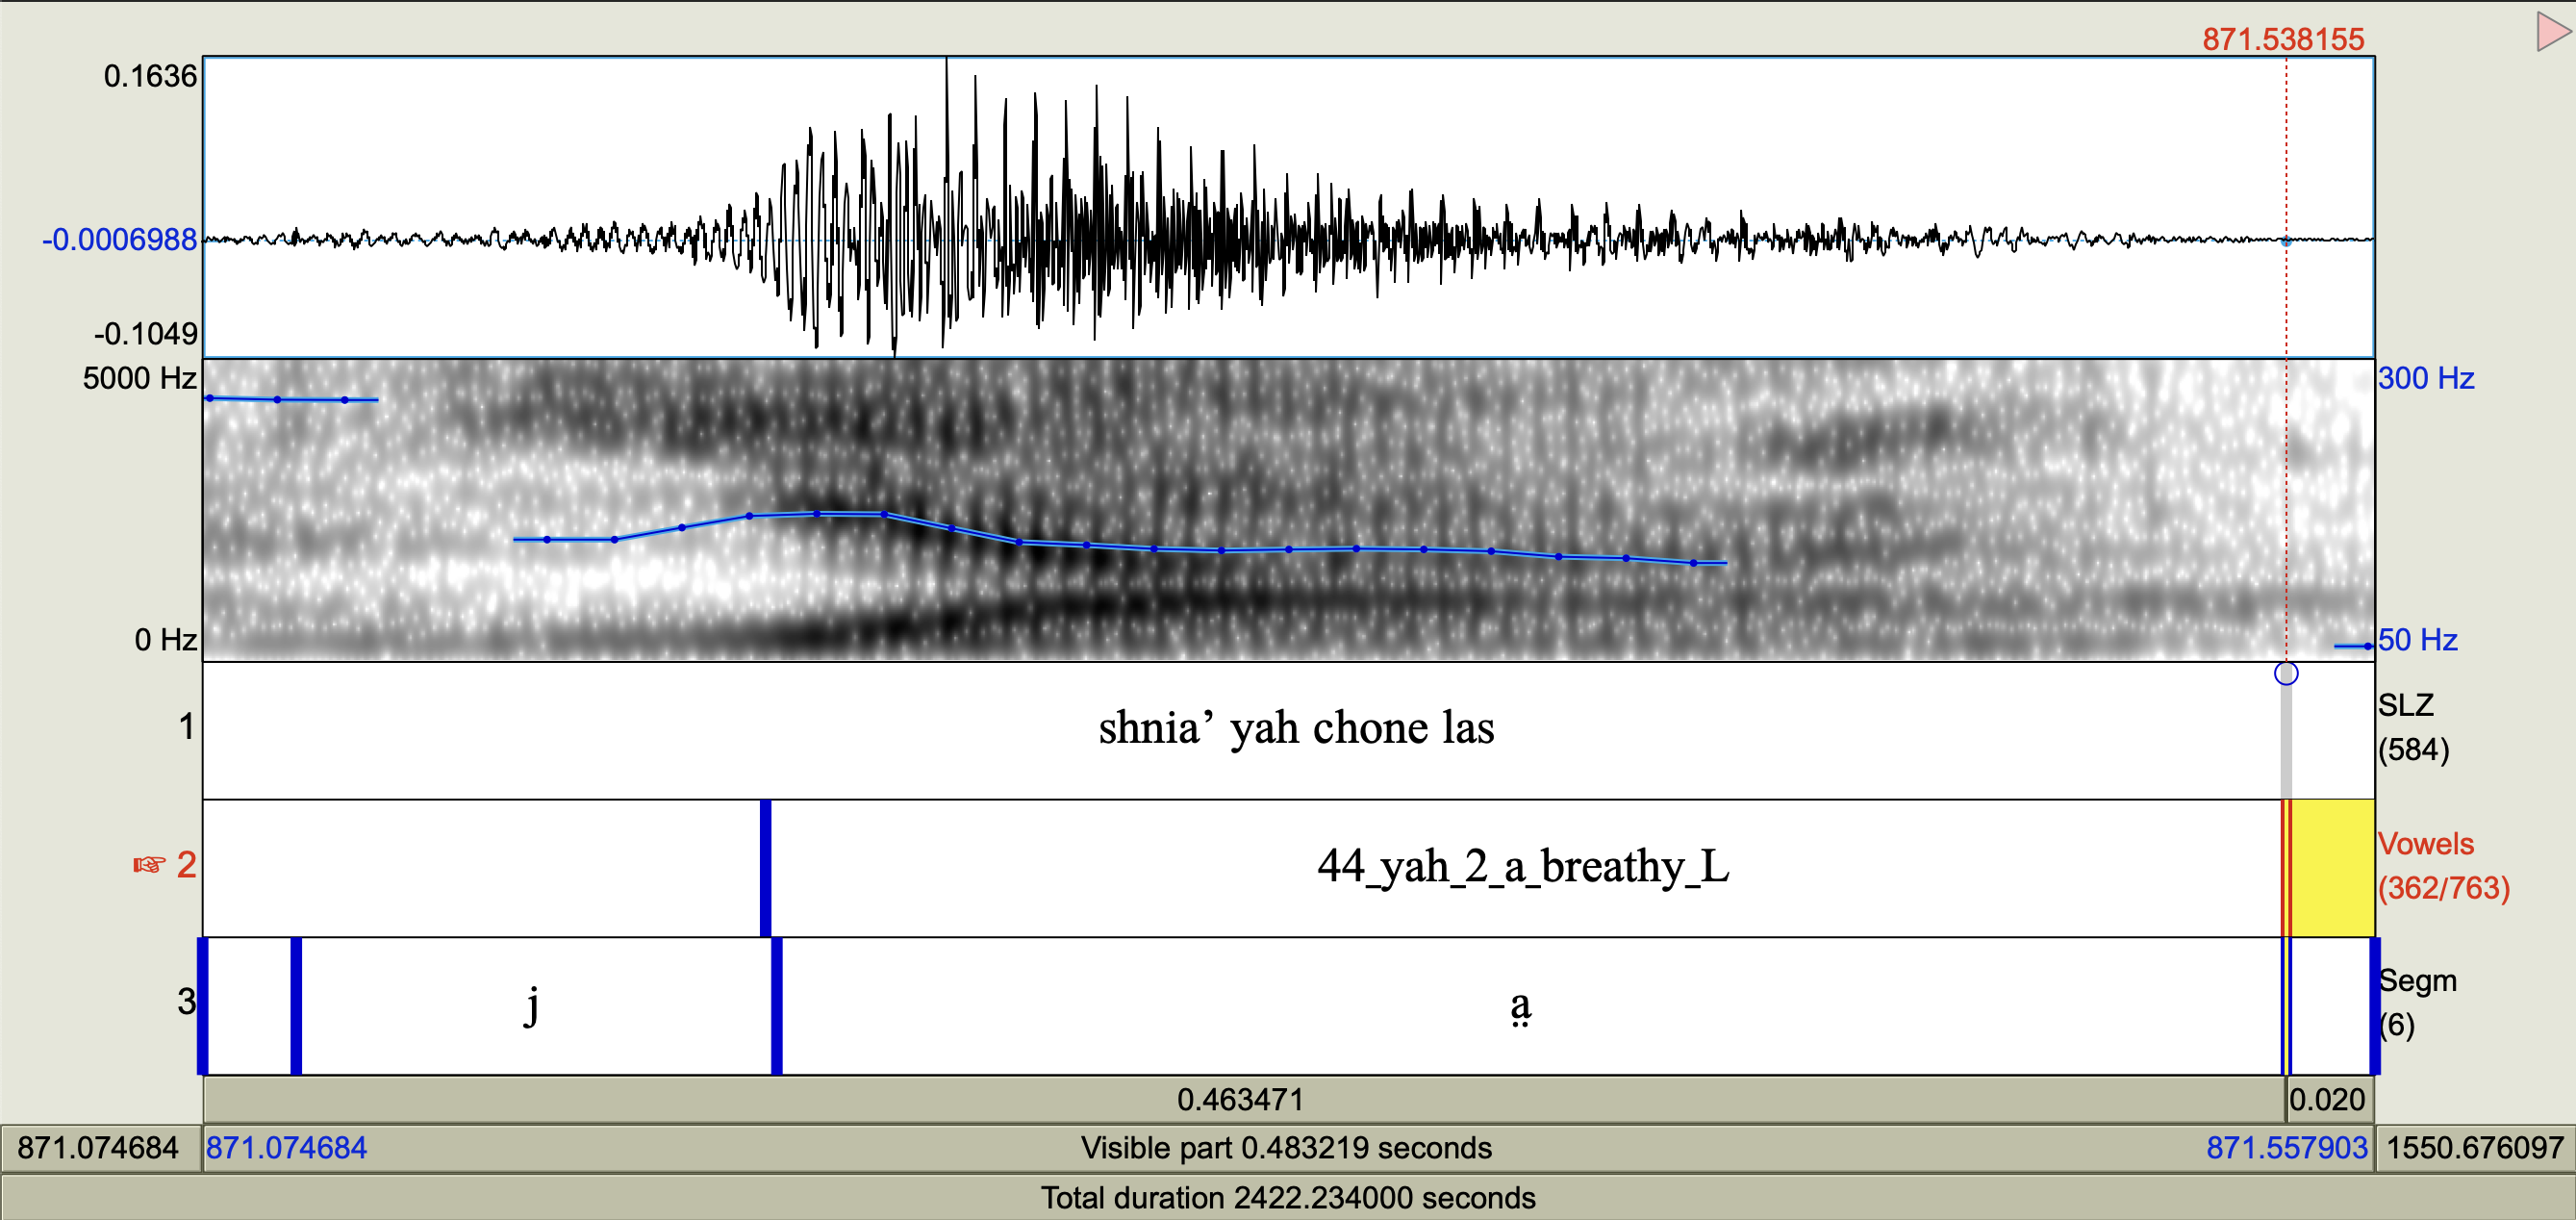
\includegraphics[width=0.9\textwidth]{../yah.png}
	\caption{FSR's breathy vowel in the word \textit{yah} `metal; rifle'}
	\label{fig:BreathyVowel}
\end{figure}

\begin{itemize}
	\item Checked vowels on the other hand are characterized by an abrupt glottal closure which cuts the vowel short. This phonation is sometimes only realized as a very short period of creakiness at the end of the vowel, see Figure~\ref{fig:CheckedVowel}.  
\end{itemize}

\begin{figure}[!h]
	\centering
	% [INSERT YA SPECTROGRAM AND WAVEFORM]
	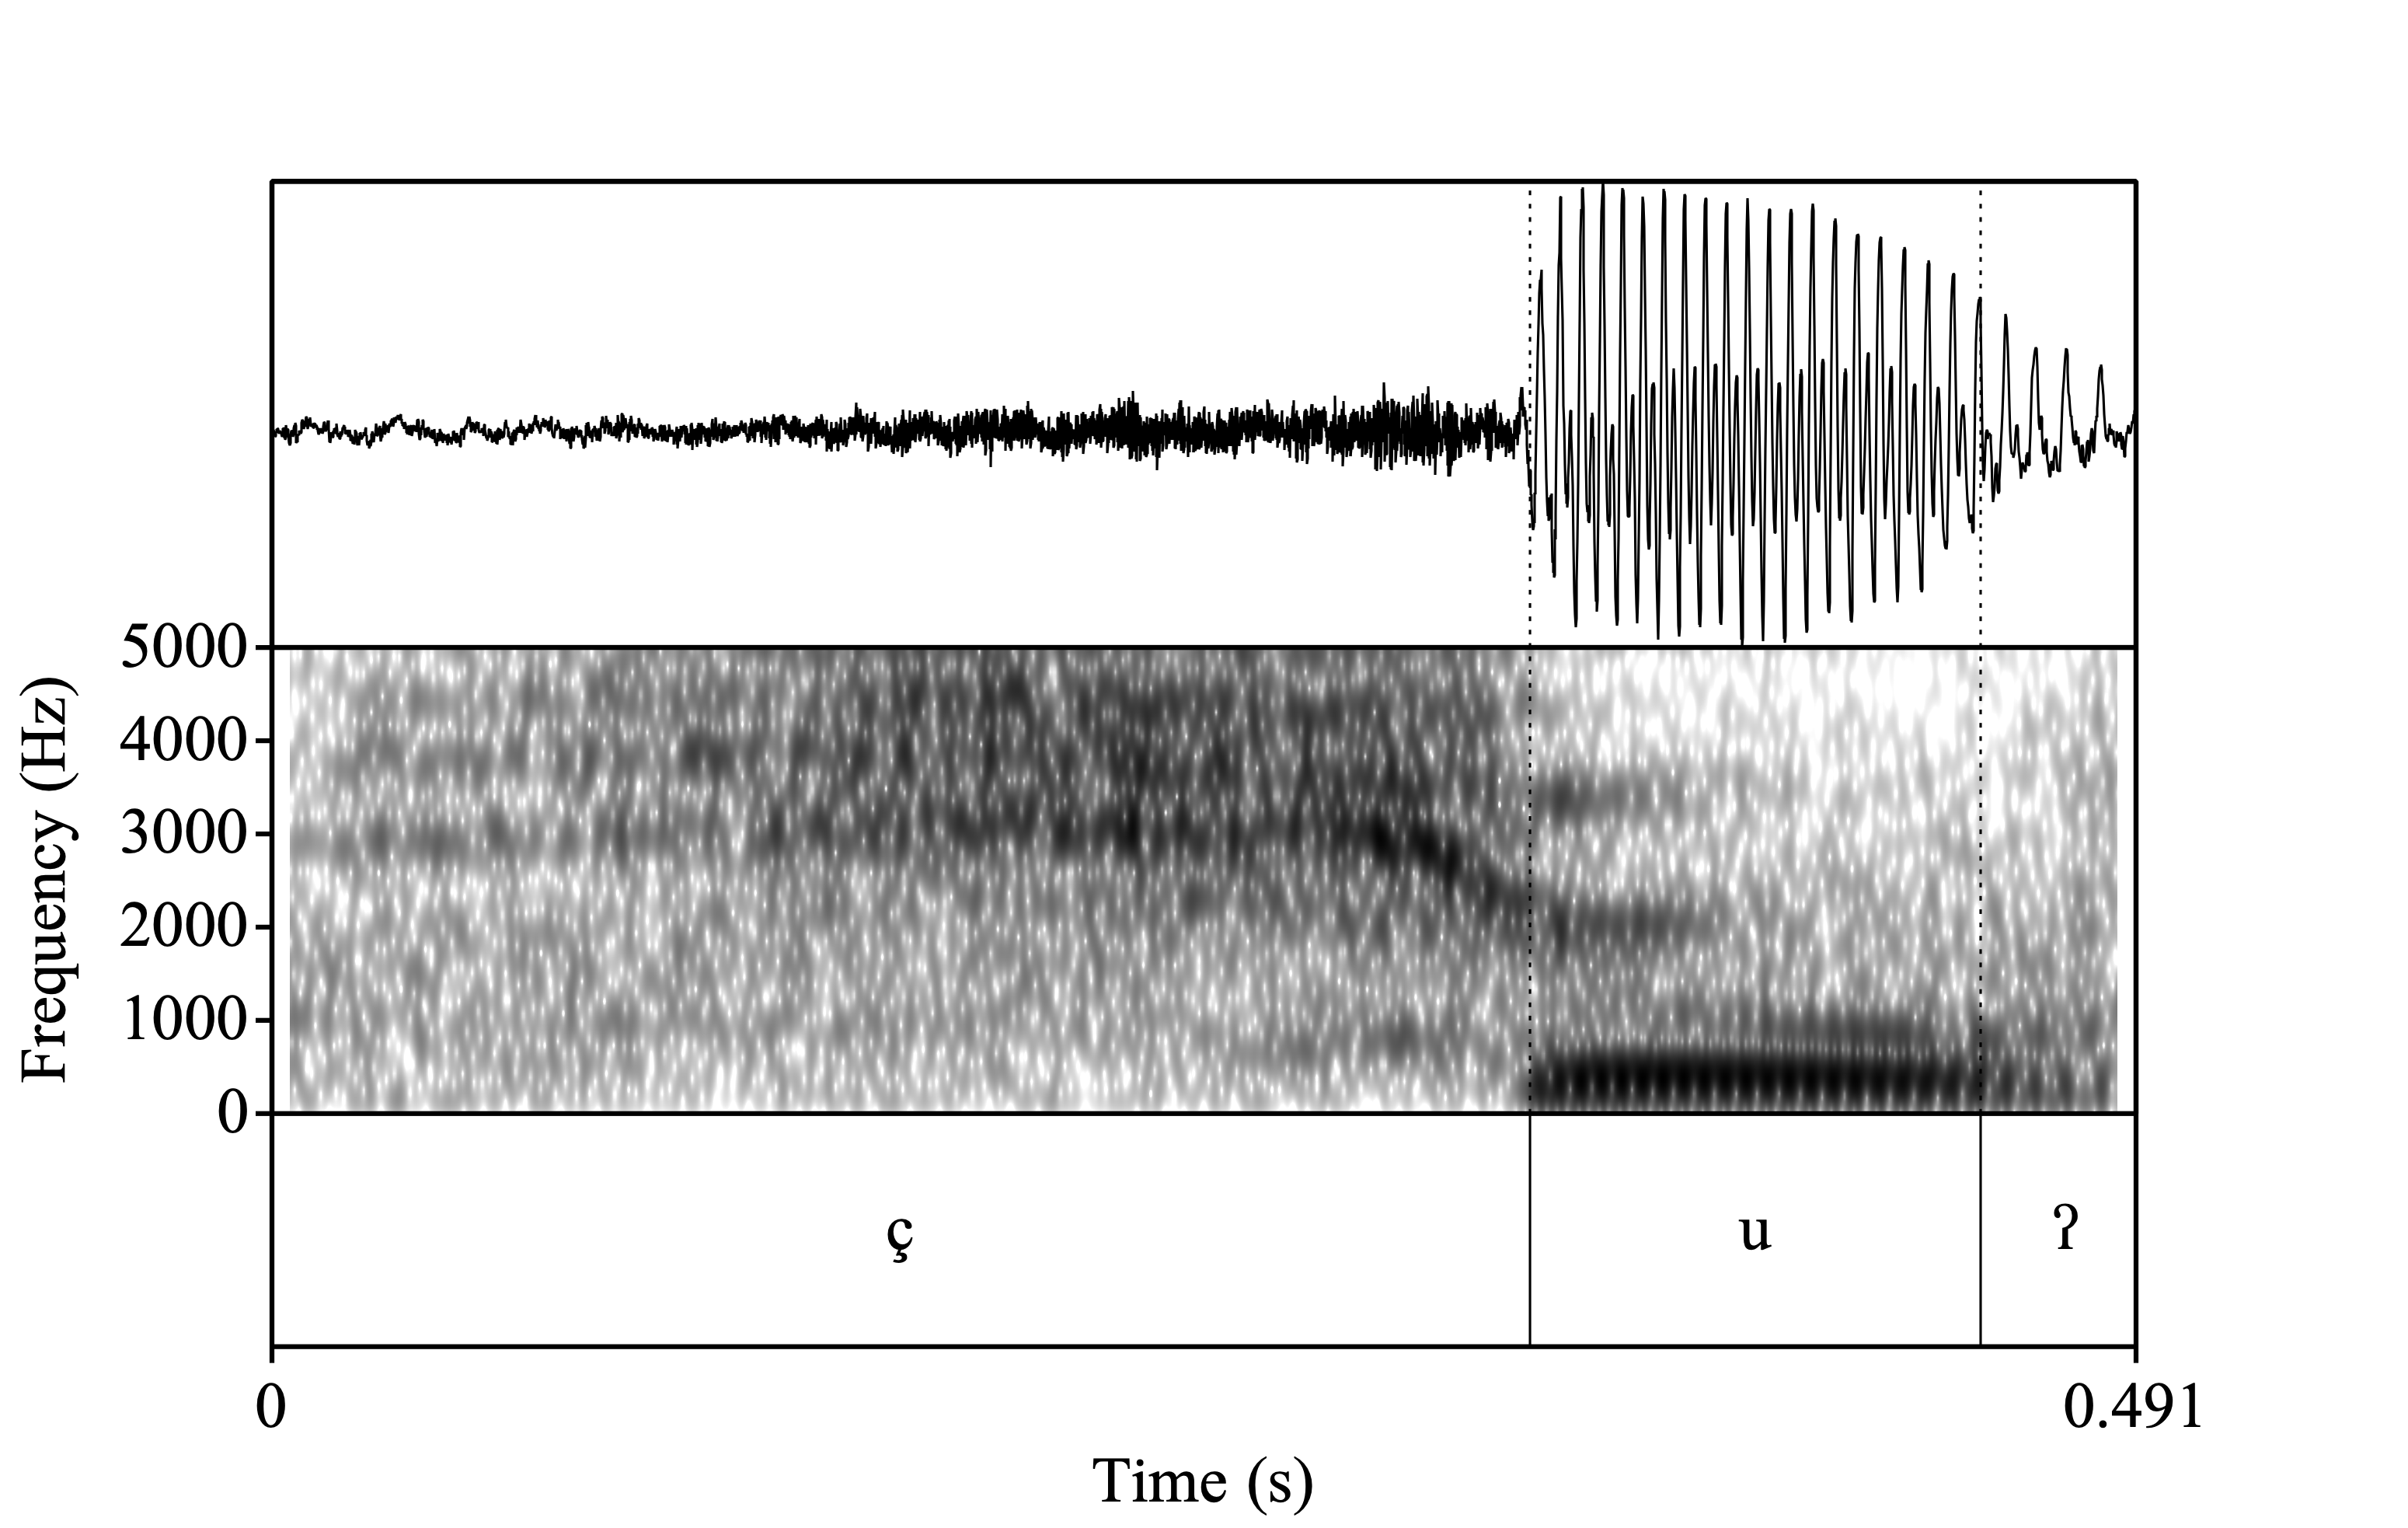
\includegraphics[width=0.9\textwidth]{../RD_yu'.png}
	\caption{RD's checked vowel in the word \textit{yu'} `earth'}
	\label{fig:CheckedVowel}
\end{figure}

\begin{itemize}
	\item Laryngealized vowels are quite common in Zapotecan languages and have received a wide number of different names. 
	\item Previous descriptions have used terms such as broken, rearticulated, interrupted, and creaky \citep{longDiccionarioZapotecoSan2005,avelinobecerraTopicsYalalagZapotec2004,avelinoAcousticElectroglottographicAnalyses2010,sonnenscheinDescriptiveGrammarSan2005,adlerAcousticsPhonationTypes2016,ariza-garciaPhonationTypesTones2018}.  
	\item In addition to a wide number of different names these vowels also exhibit a wide range of allophones.
	\item \citet{avelinoAcousticElectroglottographicAnalyses2010} found in the closely realted Yalálag Zapotec that among his consultants there were at least four different pronunciations as seen in Table~\ref{tab:laryngeal}. 
\end{itemize}

\begin{table}[!h]
	\centering
	\caption{Layngealized Vowels in Yalálag Zapotec}
	\label{tab:laryngeal}
	 \begin{tabular}{ll}
	\lsptoprule
	/VˀV/	&  [VʔV]  \\
			&  [VV̰V]   \\
			&  [VV̰ːV̆]  \\
			&  [VV̰V̰]	\\
	\lspbottomrule
	\end{tabular}
\end{table}

\begin{itemize}
	\item In SLZ, this vowel is also highly variable.
	\item One consultant does rearticulation, where there is a full glottal stop in the middle of the vowel, or creaky voice. 
	\item This alternation seemed to be in free variation but there was a greater tendency to creak in words with a L tone, such as \textit{xa'ag} [ʂa̰ːx] `topil'\footnote{A topil is a type of government office in traditional Oaxacan communities somewhat akin to a sheriff. }, see Figure~\ref{fig:FSRLaryngeal} for a comparison between this consultant's pronunciation of the laryngealized vowels.
\end{itemize}

\begin{figure}[!h]
	\centering
	\begin{subfigure}{.5\textwidth}
		\centering
		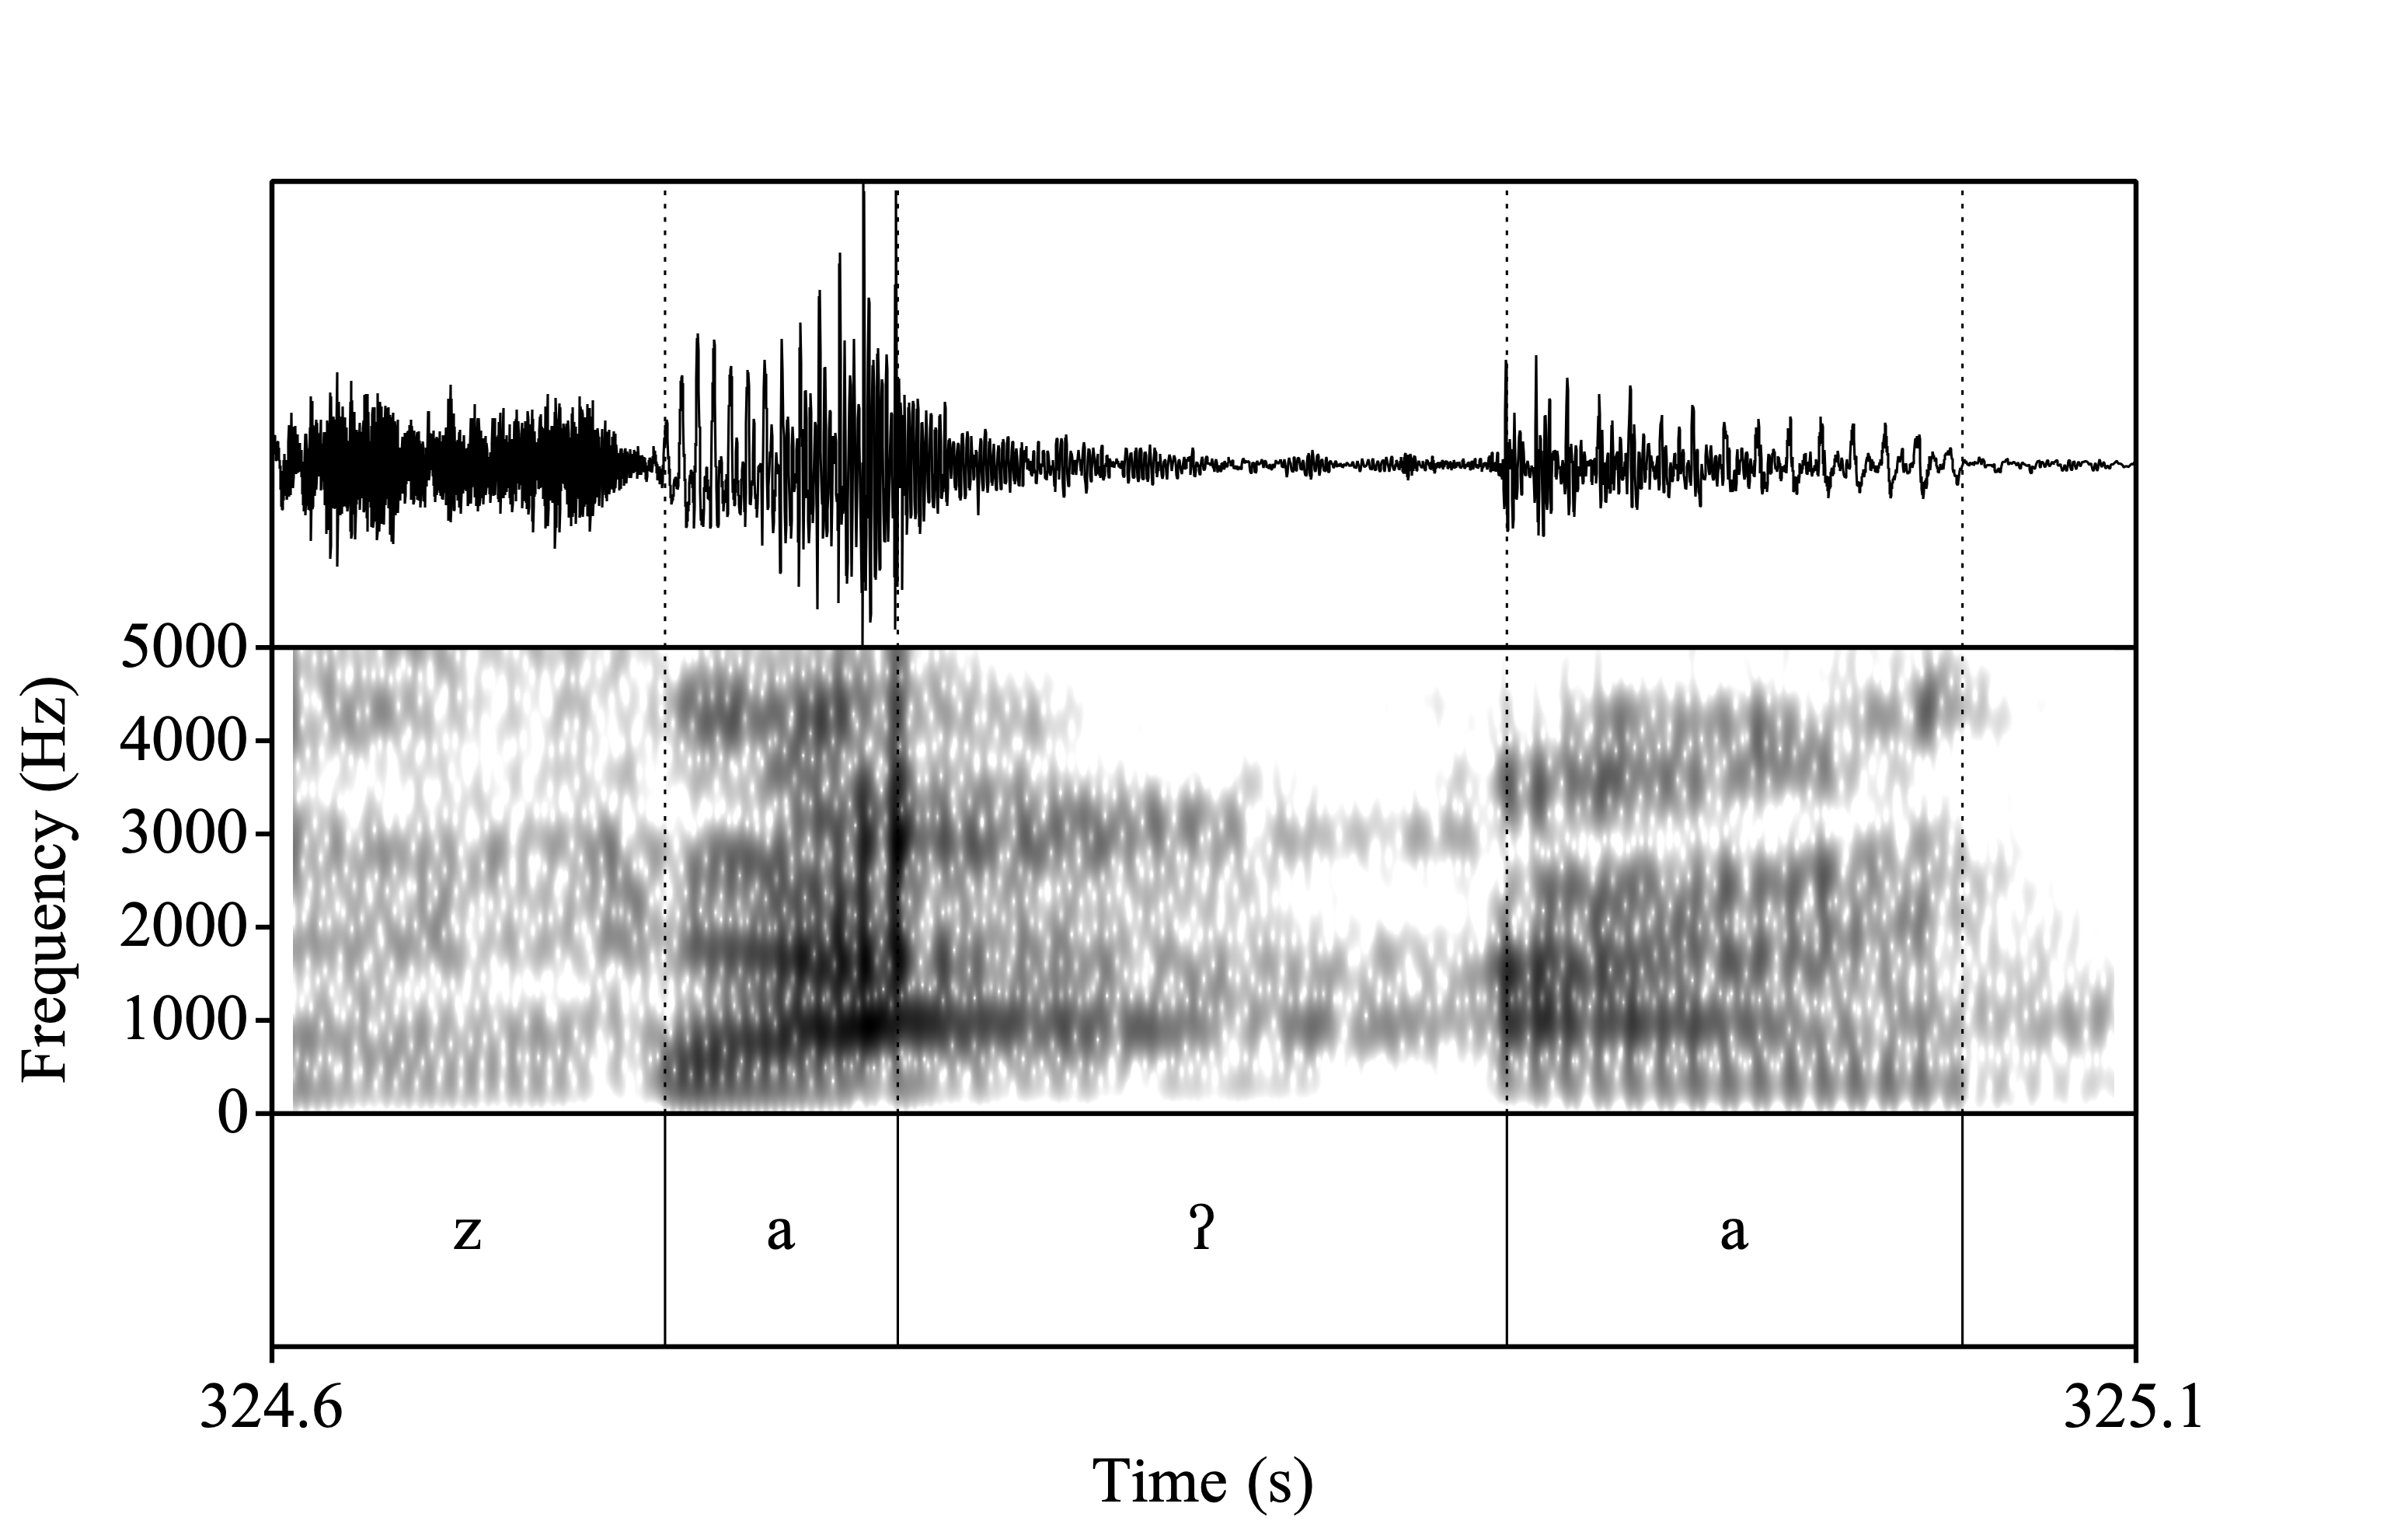
\includegraphics[width=\linewidth]{../za'a.png}
		\caption{\textit{za'a} `corncob'}
		\label{fig:za'a}
	\end{subfigure}%
	\begin{subfigure}{.5\textwidth}
		\centering
		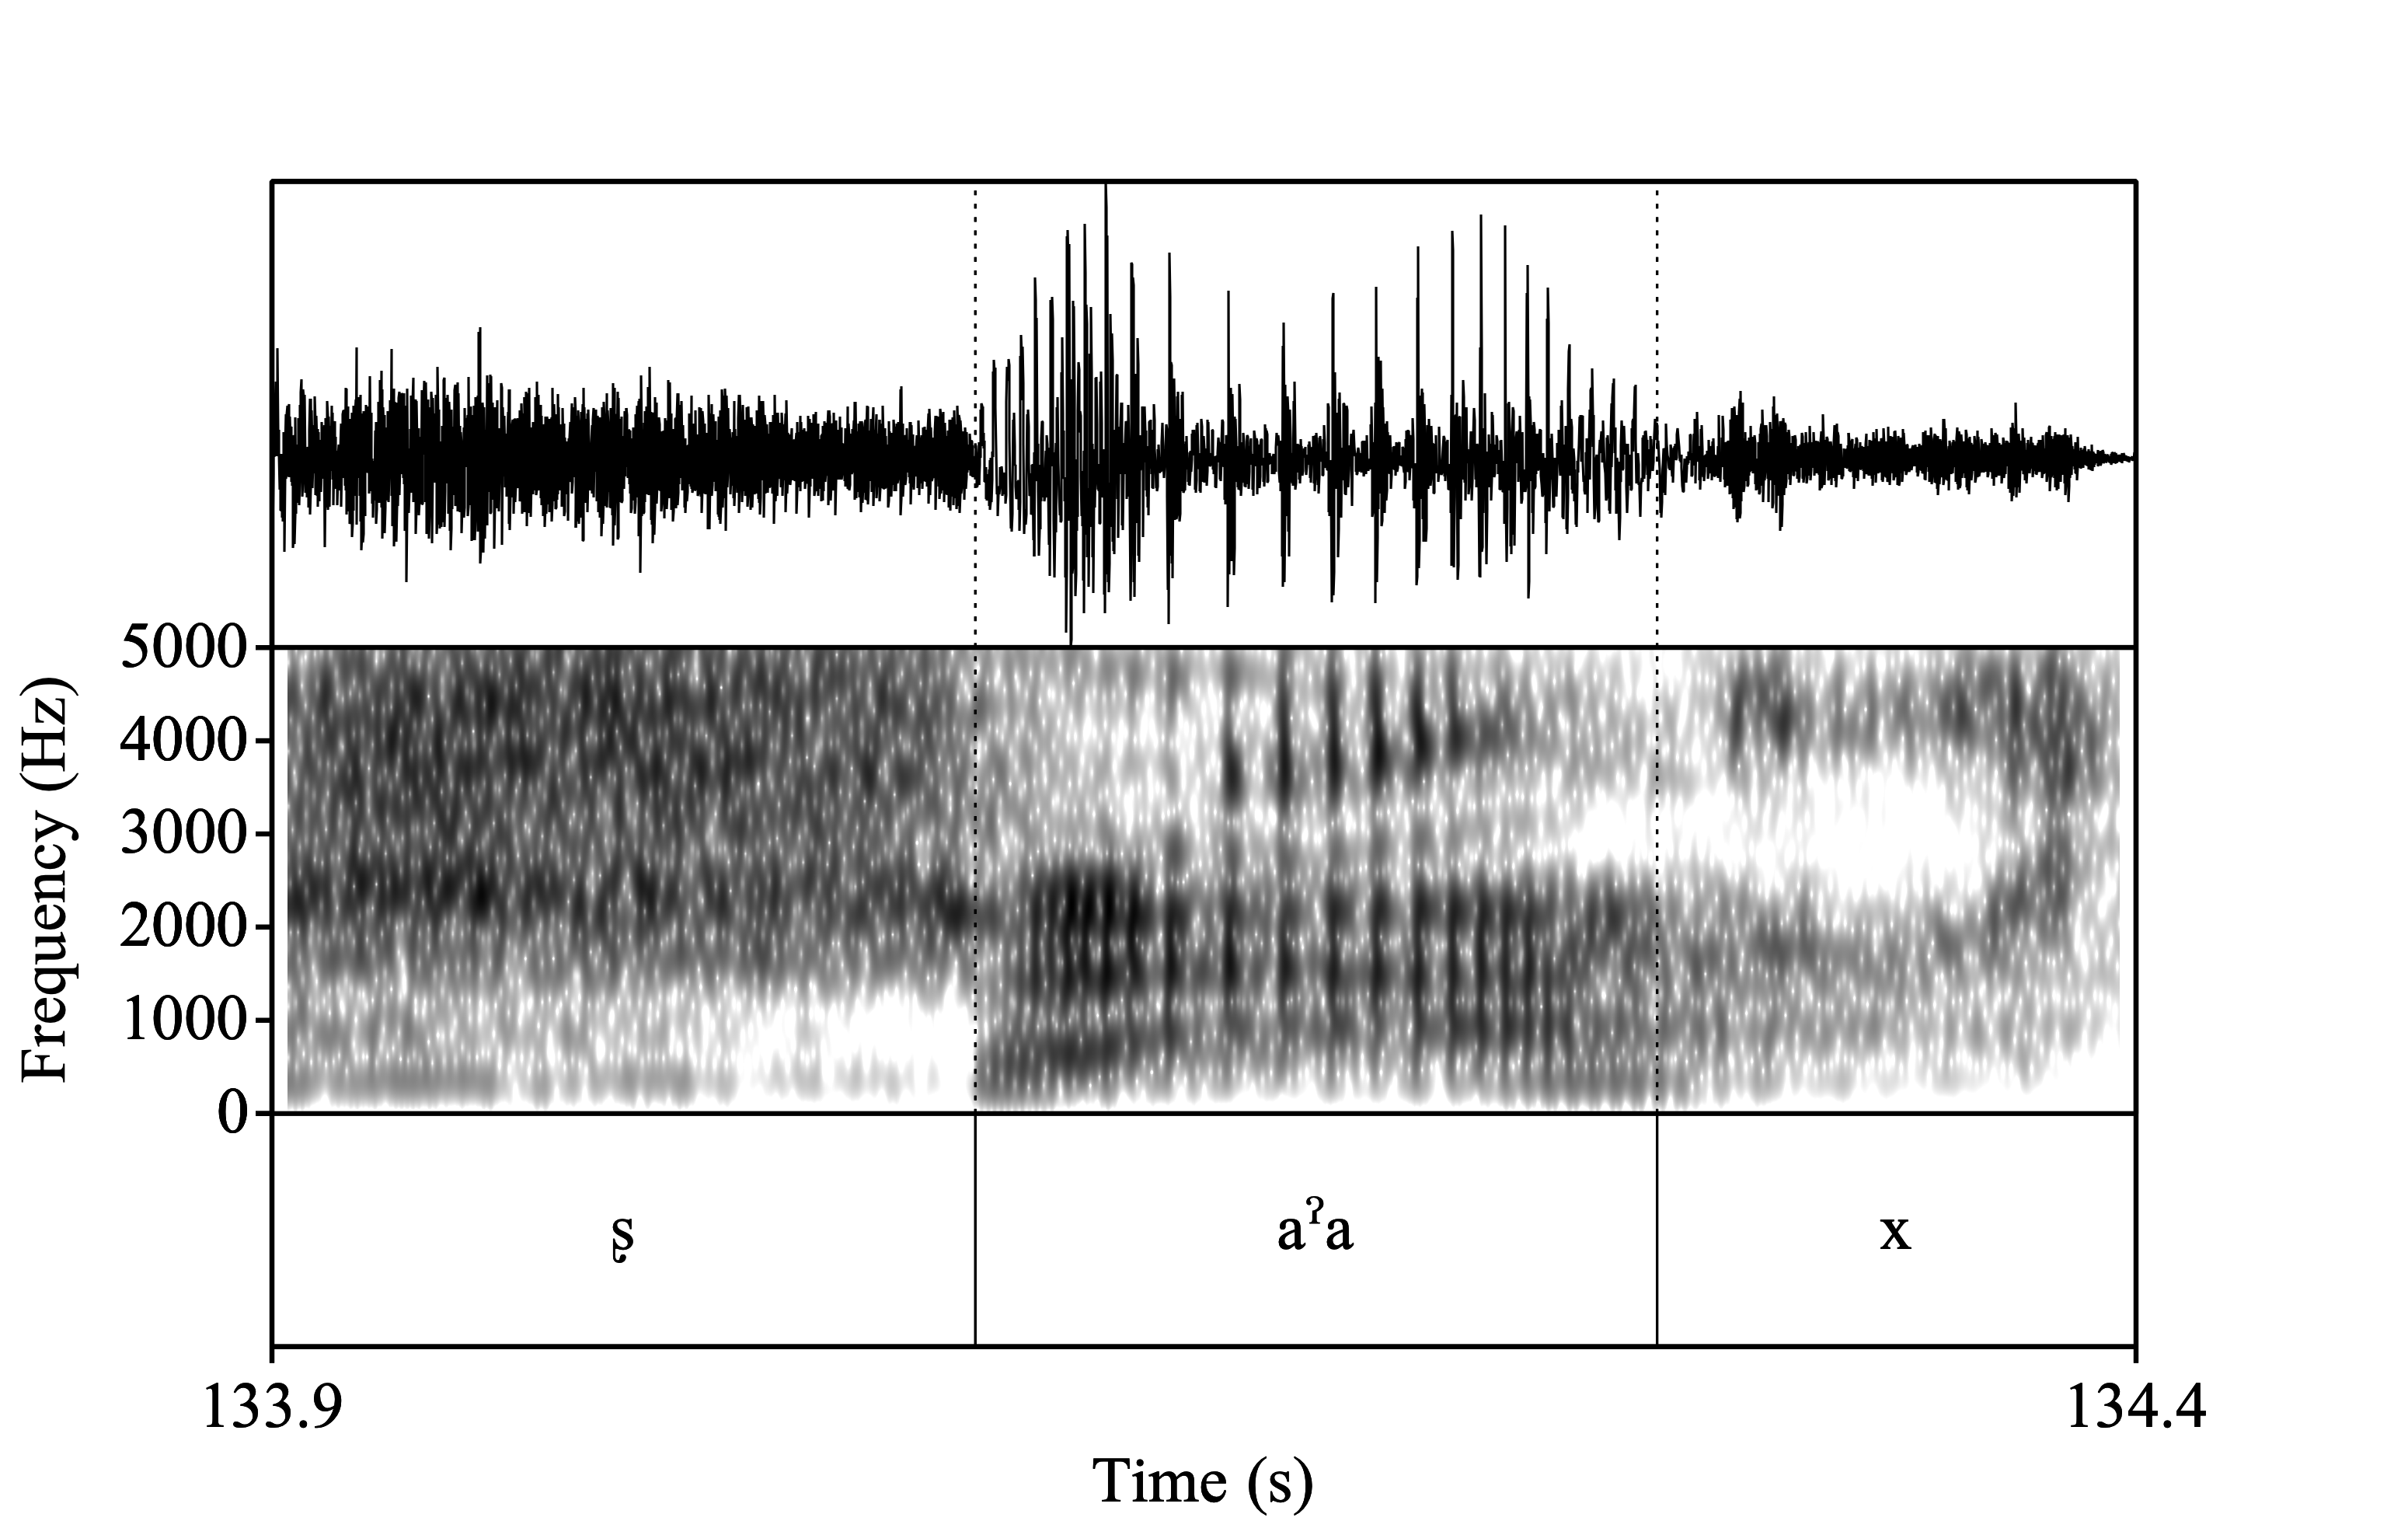
\includegraphics[width=\linewidth]{../xa'ag.png}
		\caption{\textit{xa'ag} `topil'}
		\label{fig:xa'ag}
	\end{subfigure}	
	\caption{Comparison of FSR's laryngealized vowels in \textit{za'a} `corncob' and \textit{xa'ag} `topil'}
	\label{fig:FSRLaryngeal}
\end{figure}

\begin{itemize}
	\item Another consultant only ever produces creaky voice for these vowels regardless of the tone with the word.
\end{itemize}

\begin{figure}[!h]
	\centering
	\begin{subfigure}{.5\textwidth}
		\centering
		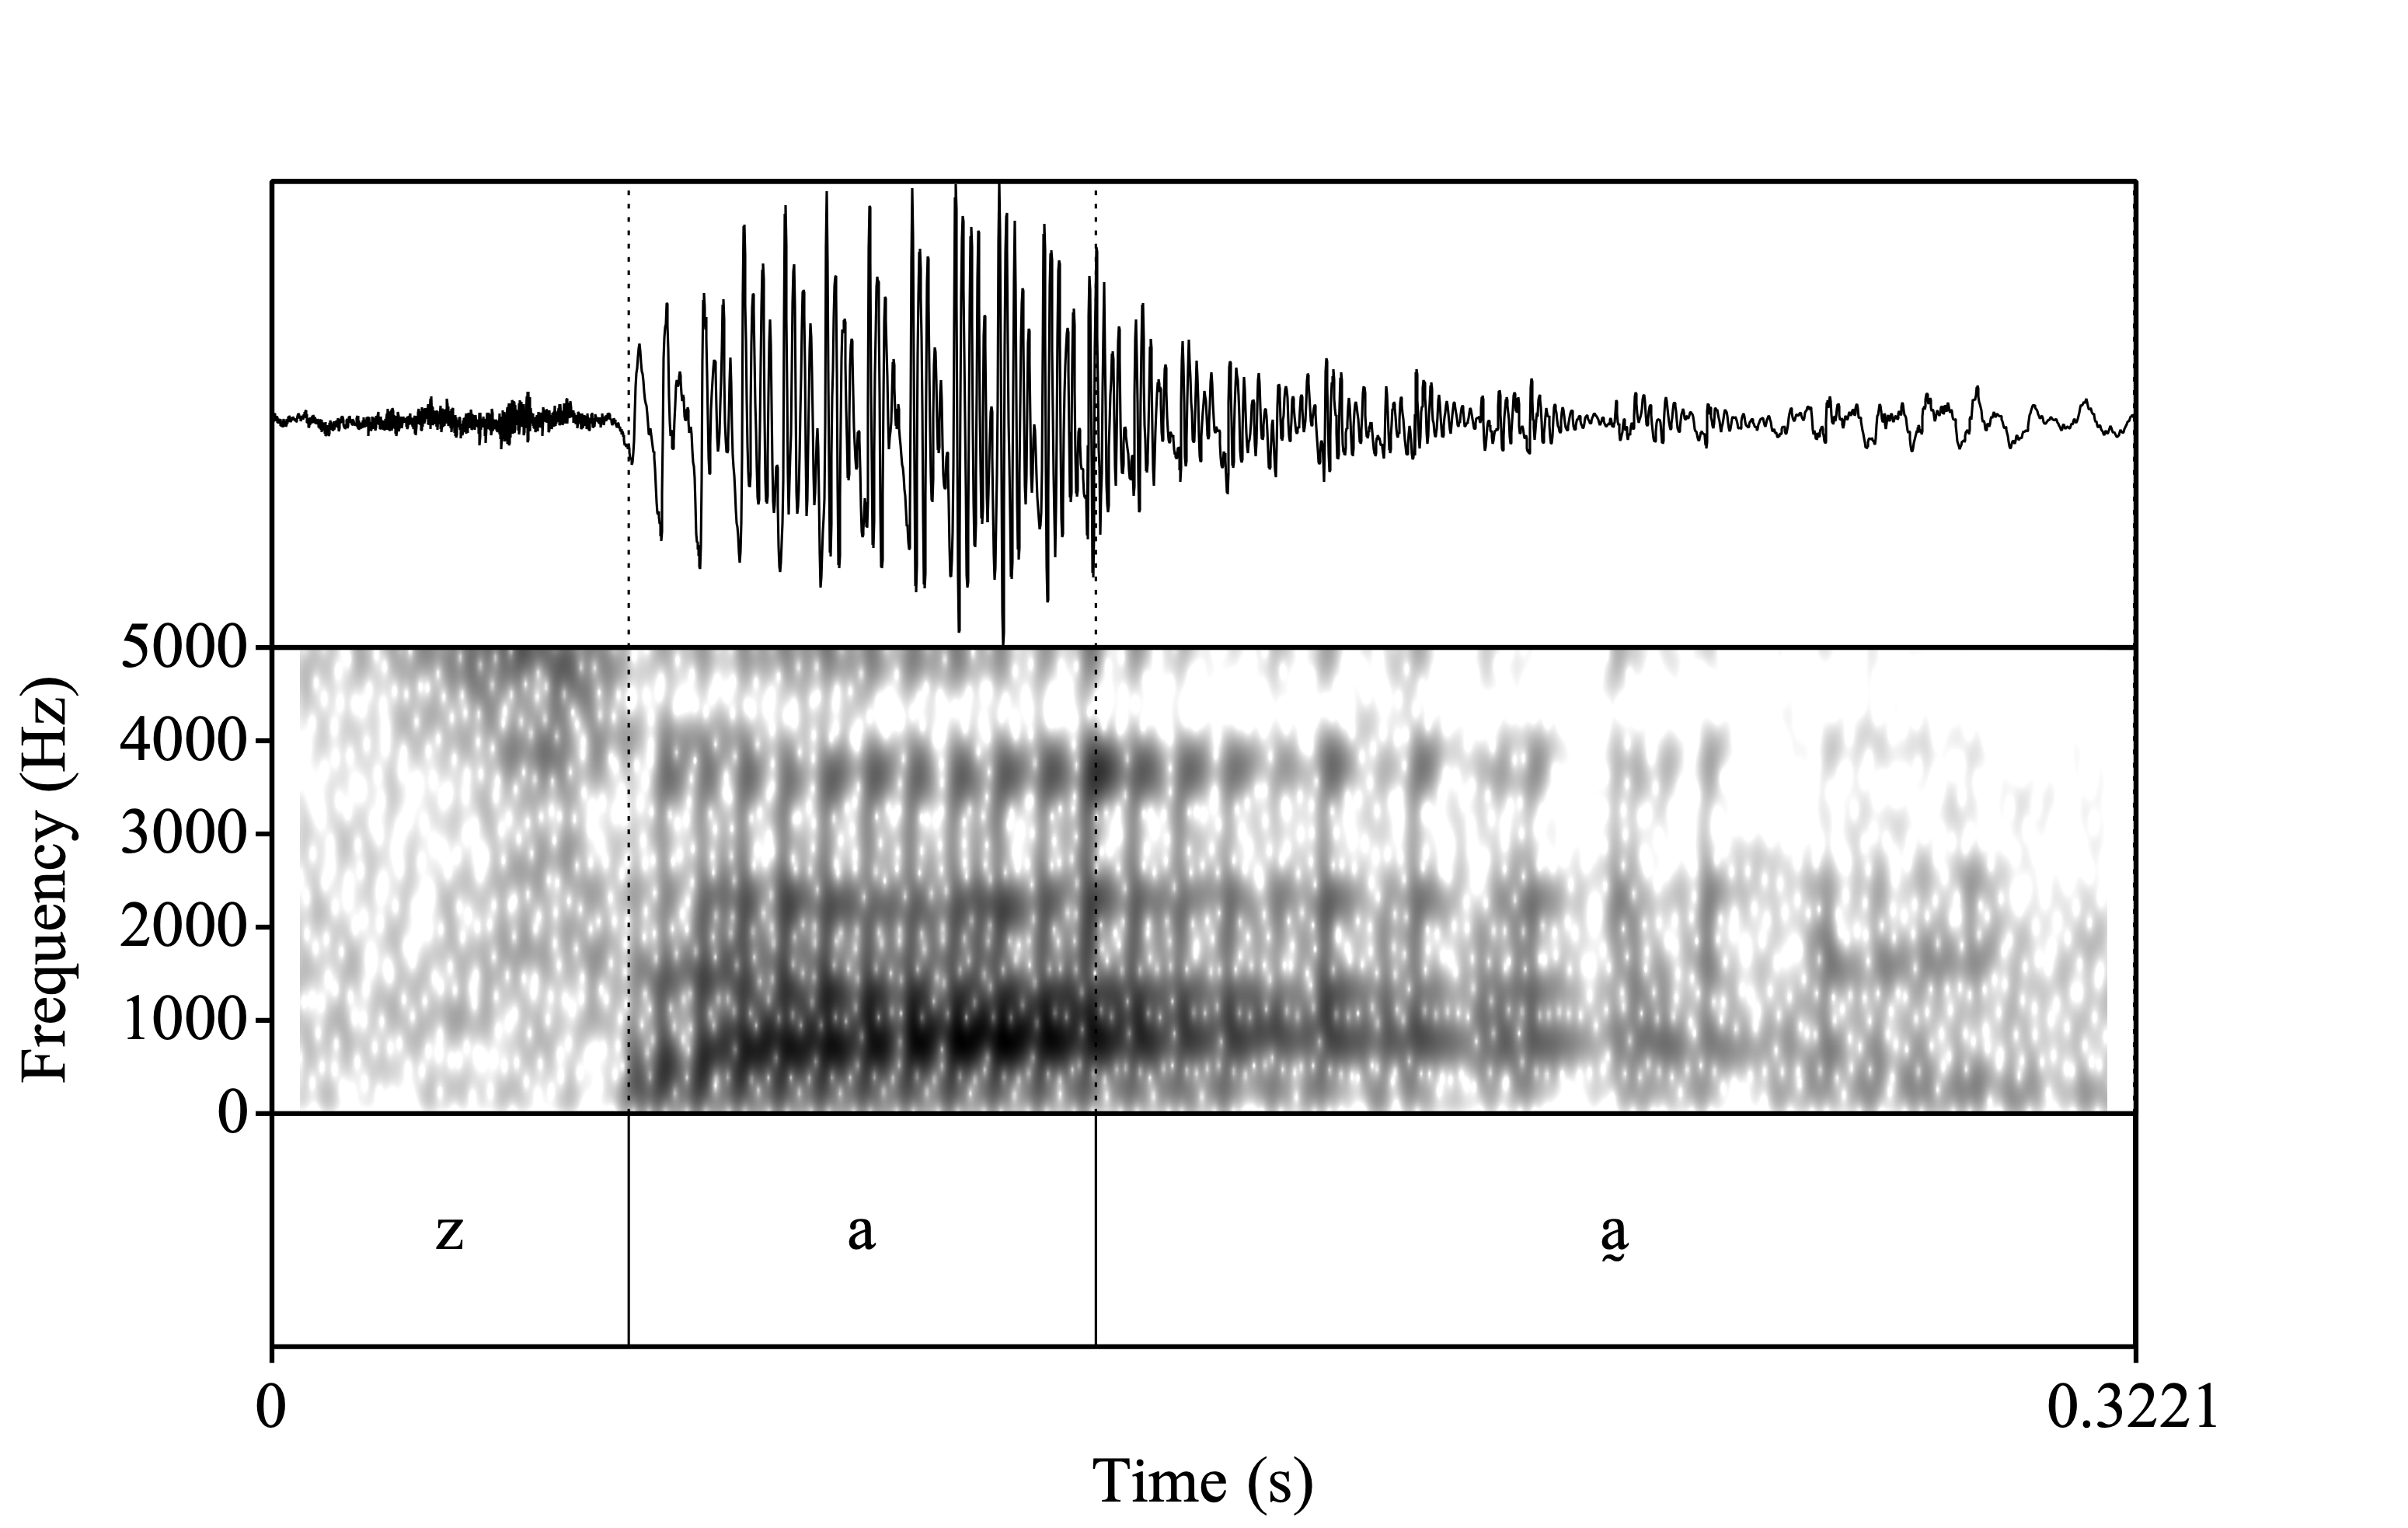
\includegraphics[width=\linewidth]{../RD_za'a.png}
		\caption{\textit{za'a} `corncob'}
		\label{fig:za'a}
	\end{subfigure}%
	\begin{subfigure}{.5\textwidth}
		\centering
		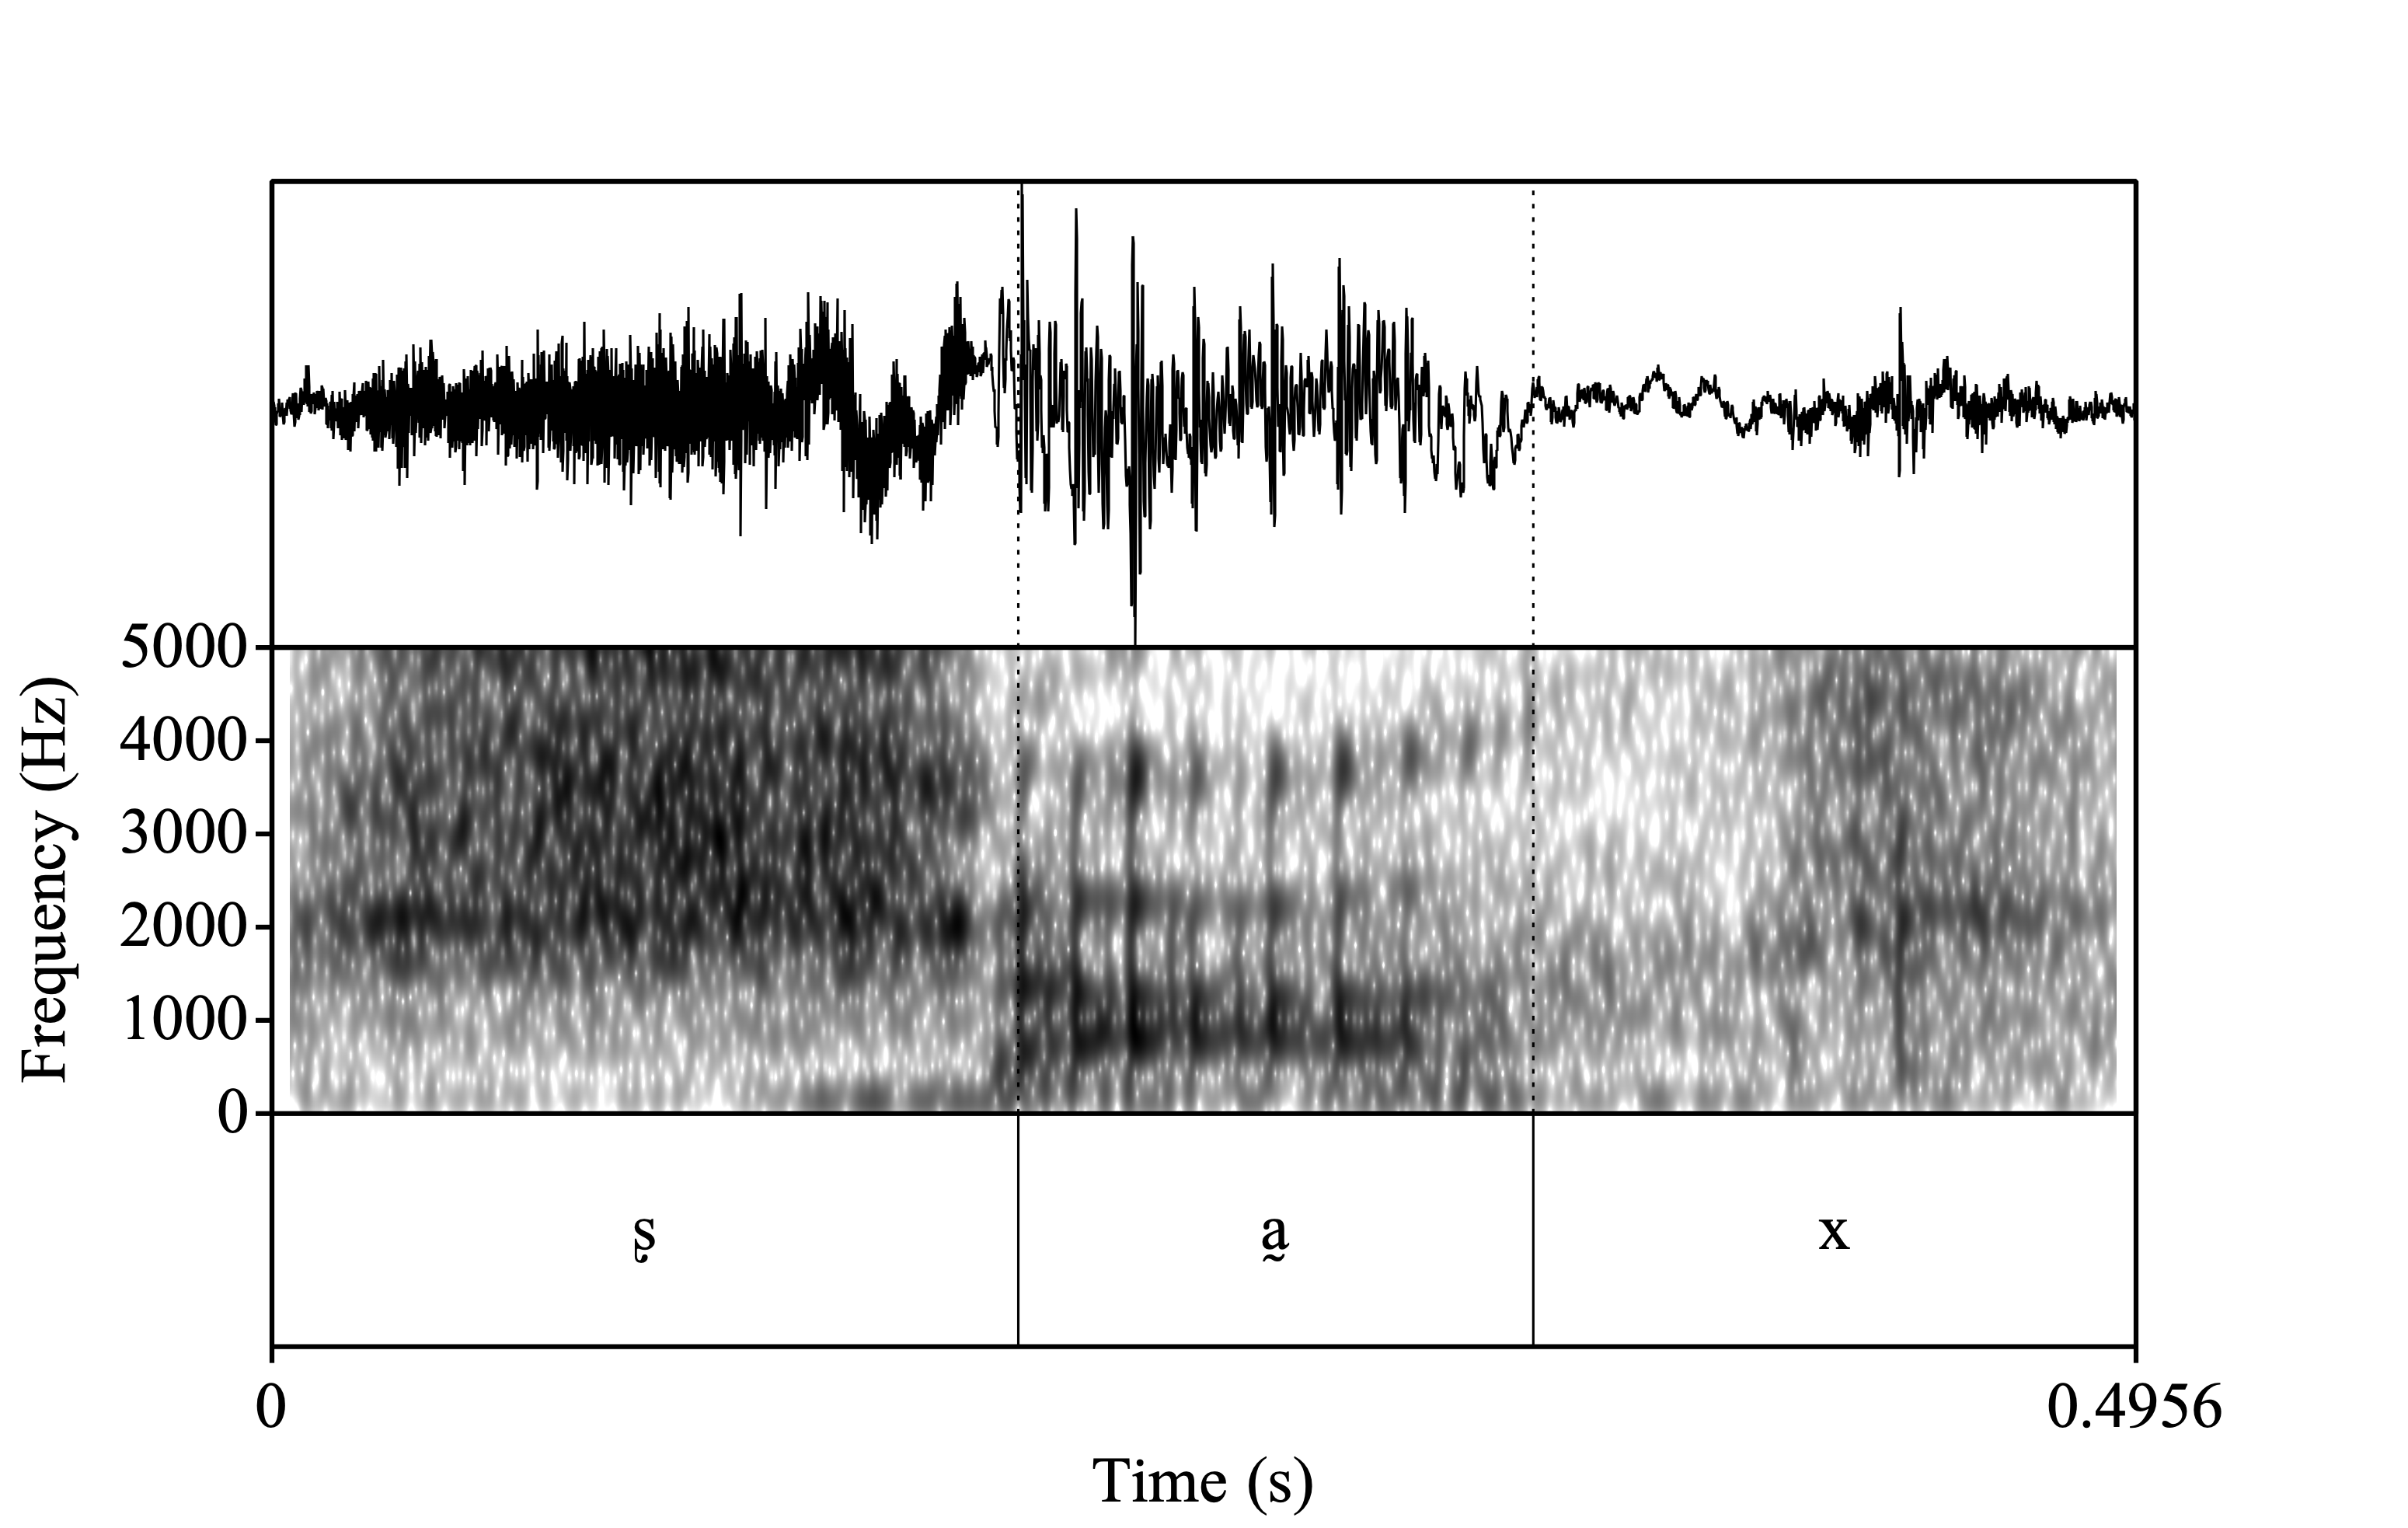
\includegraphics[width=\linewidth]{../RD_xa'ag.png}
		\caption{\textit{xa'ag} `topil'}
		\label{fig:xa'ag}
	\end{subfigure}
	\caption{Comparison of RD's laryngealized vowels in \textit{za'a} `corncob' and \textit{xa'ag} `topil'}
	\label{fig:RDLaryngeal}
\end{figure}

%------------------------------------
\subsection{Interaction of tone and phonation in Santiago Laxopa Zapotec} \label{sec:TonePhonation}
%------------------------------------

\begin{table}[!ht]
	\centering
	\caption{SLQZ tone and phonation interactions \citep{chavez-peonInteractionMetricalStructure2010}.}
	\label{tab:SLQZ}
	 \begin{tabular}{lcccc}
	  \lsptoprule
					  &	 \textbf{Modal}  & \textbf{Breathy} & \textbf{Creaky} & \textbf{Interrupted} \\
		  High	& ✔︎ & -- & ✔︎ & ✔︎ \\
		  Low & ✔︎ & ✔︎ & ✔︎ & ✔︎ \\
		  Falling & ✔︎ & ✔︎ & ✔︎ & ✔︎ \\
		  Rising & ✔︎ & -- & -- & -- \\
	  \lspbottomrule
	 \end{tabular}
\end{table}

\begin{table}[!h]
	\caption{Number of unique syllables for each interaction of tone and phonation in the data.}
	\label{tab:ToneVoiceQuality}
	\centering

	\begin{tabular}{lcccc}
	\lsptoprule
		& \textbf{Modal} & \textbf{Breathy} & \textbf{Checked} & \textbf{Laryngealized} \\
	\hline
	High		& ✔︎ & -- & ✔︎ & ✔︎ \\
	Mid			& ✔︎ & ✔︎  & ✔︎ & ✔︎ \\
	Low			& ✔︎ & ✔︎  & ✔︎ & ✔︎ \\
	High-Low	& ✔︎ & ✔︎  & ✔︎ & ✔︎ \\
	Mid-High	& ✔︎ & ✔︎  & --	& ✔︎ \\
	\lspbottomrule
	\end{tabular}
\end{table}


%------------------------------------
\section{Methodology} \label{sec:Methods}
%------------------------------------

\begin{itemize}
	\item Two native language speakers of SLZ who live in Santa Cruz, CA took part in this study (one male). 
	\item Because of the COVID-19 pandemic data collection was conducted remotely using Zencastr\footnote{\href{https://zencastr.com/}{https://zencastr.com/}}, a professional podcasting website, (44.1kHz, 16-bit) or in-person outside in a well ventilated location, using a Zoom H4n handheld recorder (44.1kHz, 16-bit).
	\item The 
\end{itemize}

%------------------------------------
\section{Results} \label{sec:Results}
%------------------------------------

%------------------------------------
\subsection{H1-H2 spectral-tilt} \label{sec:H1H2}
%------------------------------------


\begin{figure}[!ht]
	\centering
	\begin{subfigure}{.5\textwidth}
		\centering
		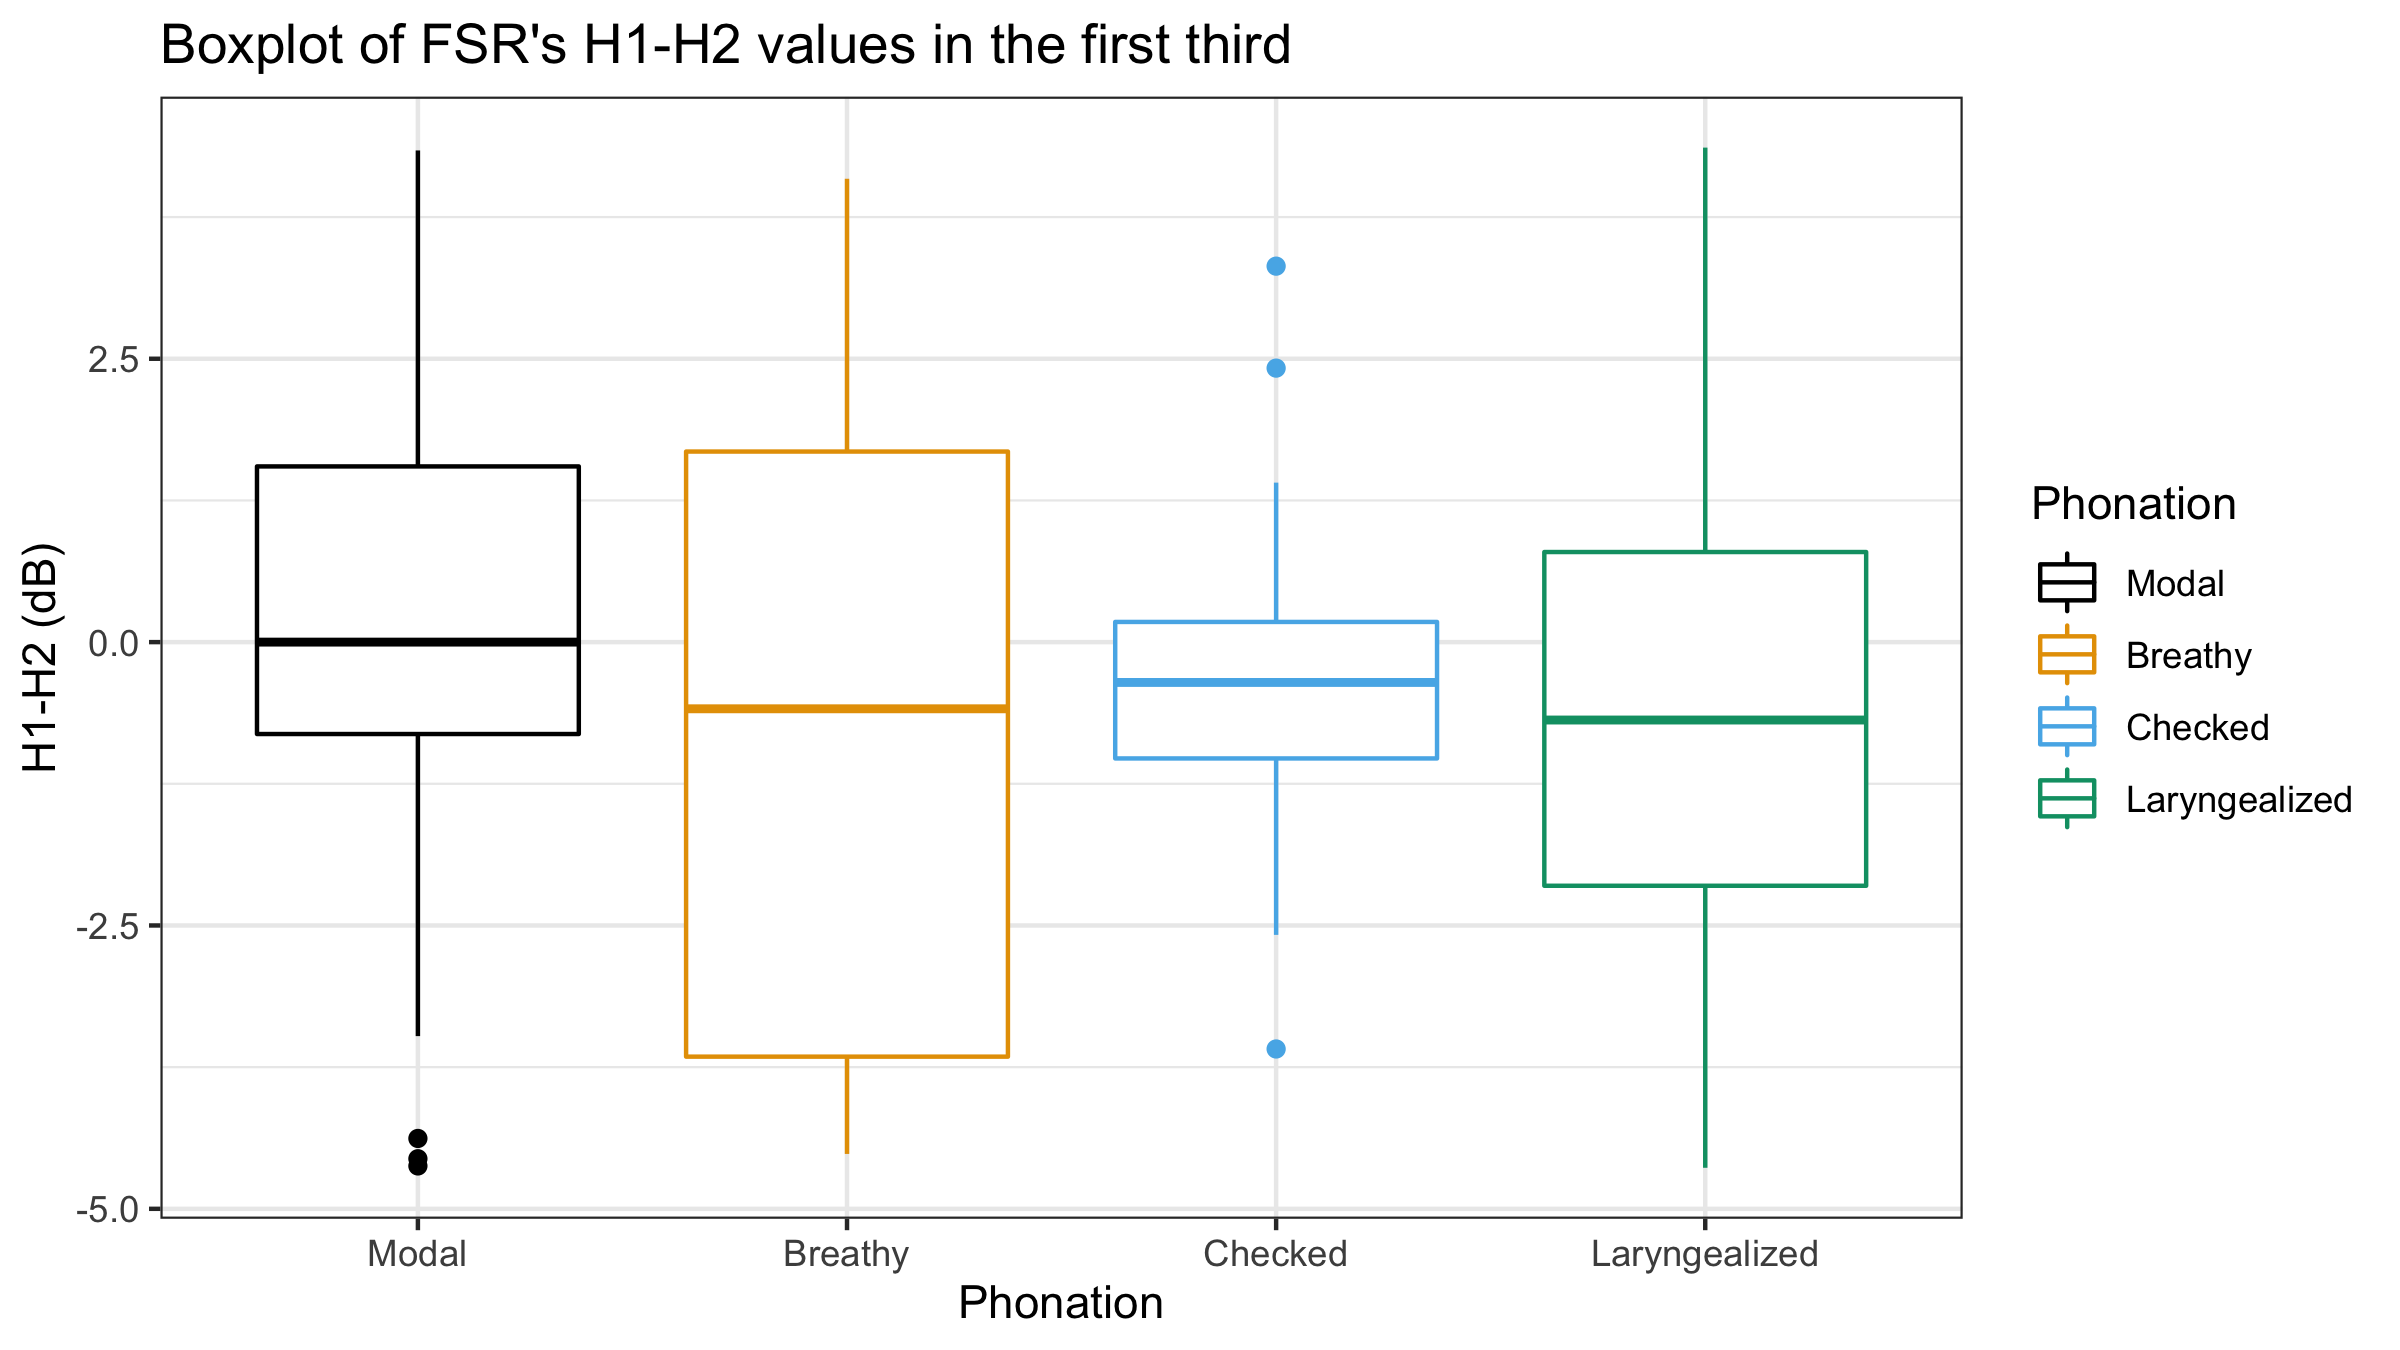
\includegraphics[width=0.9\textwidth]{../mean_FSR_h1h2_1st.png}
		\caption{FSR's H1-H2 values.}
		\label{fig:FSRh1h2first} 
	\end{subfigure}%
	\begin{subfigure}{.5\textwidth}
		\centering
		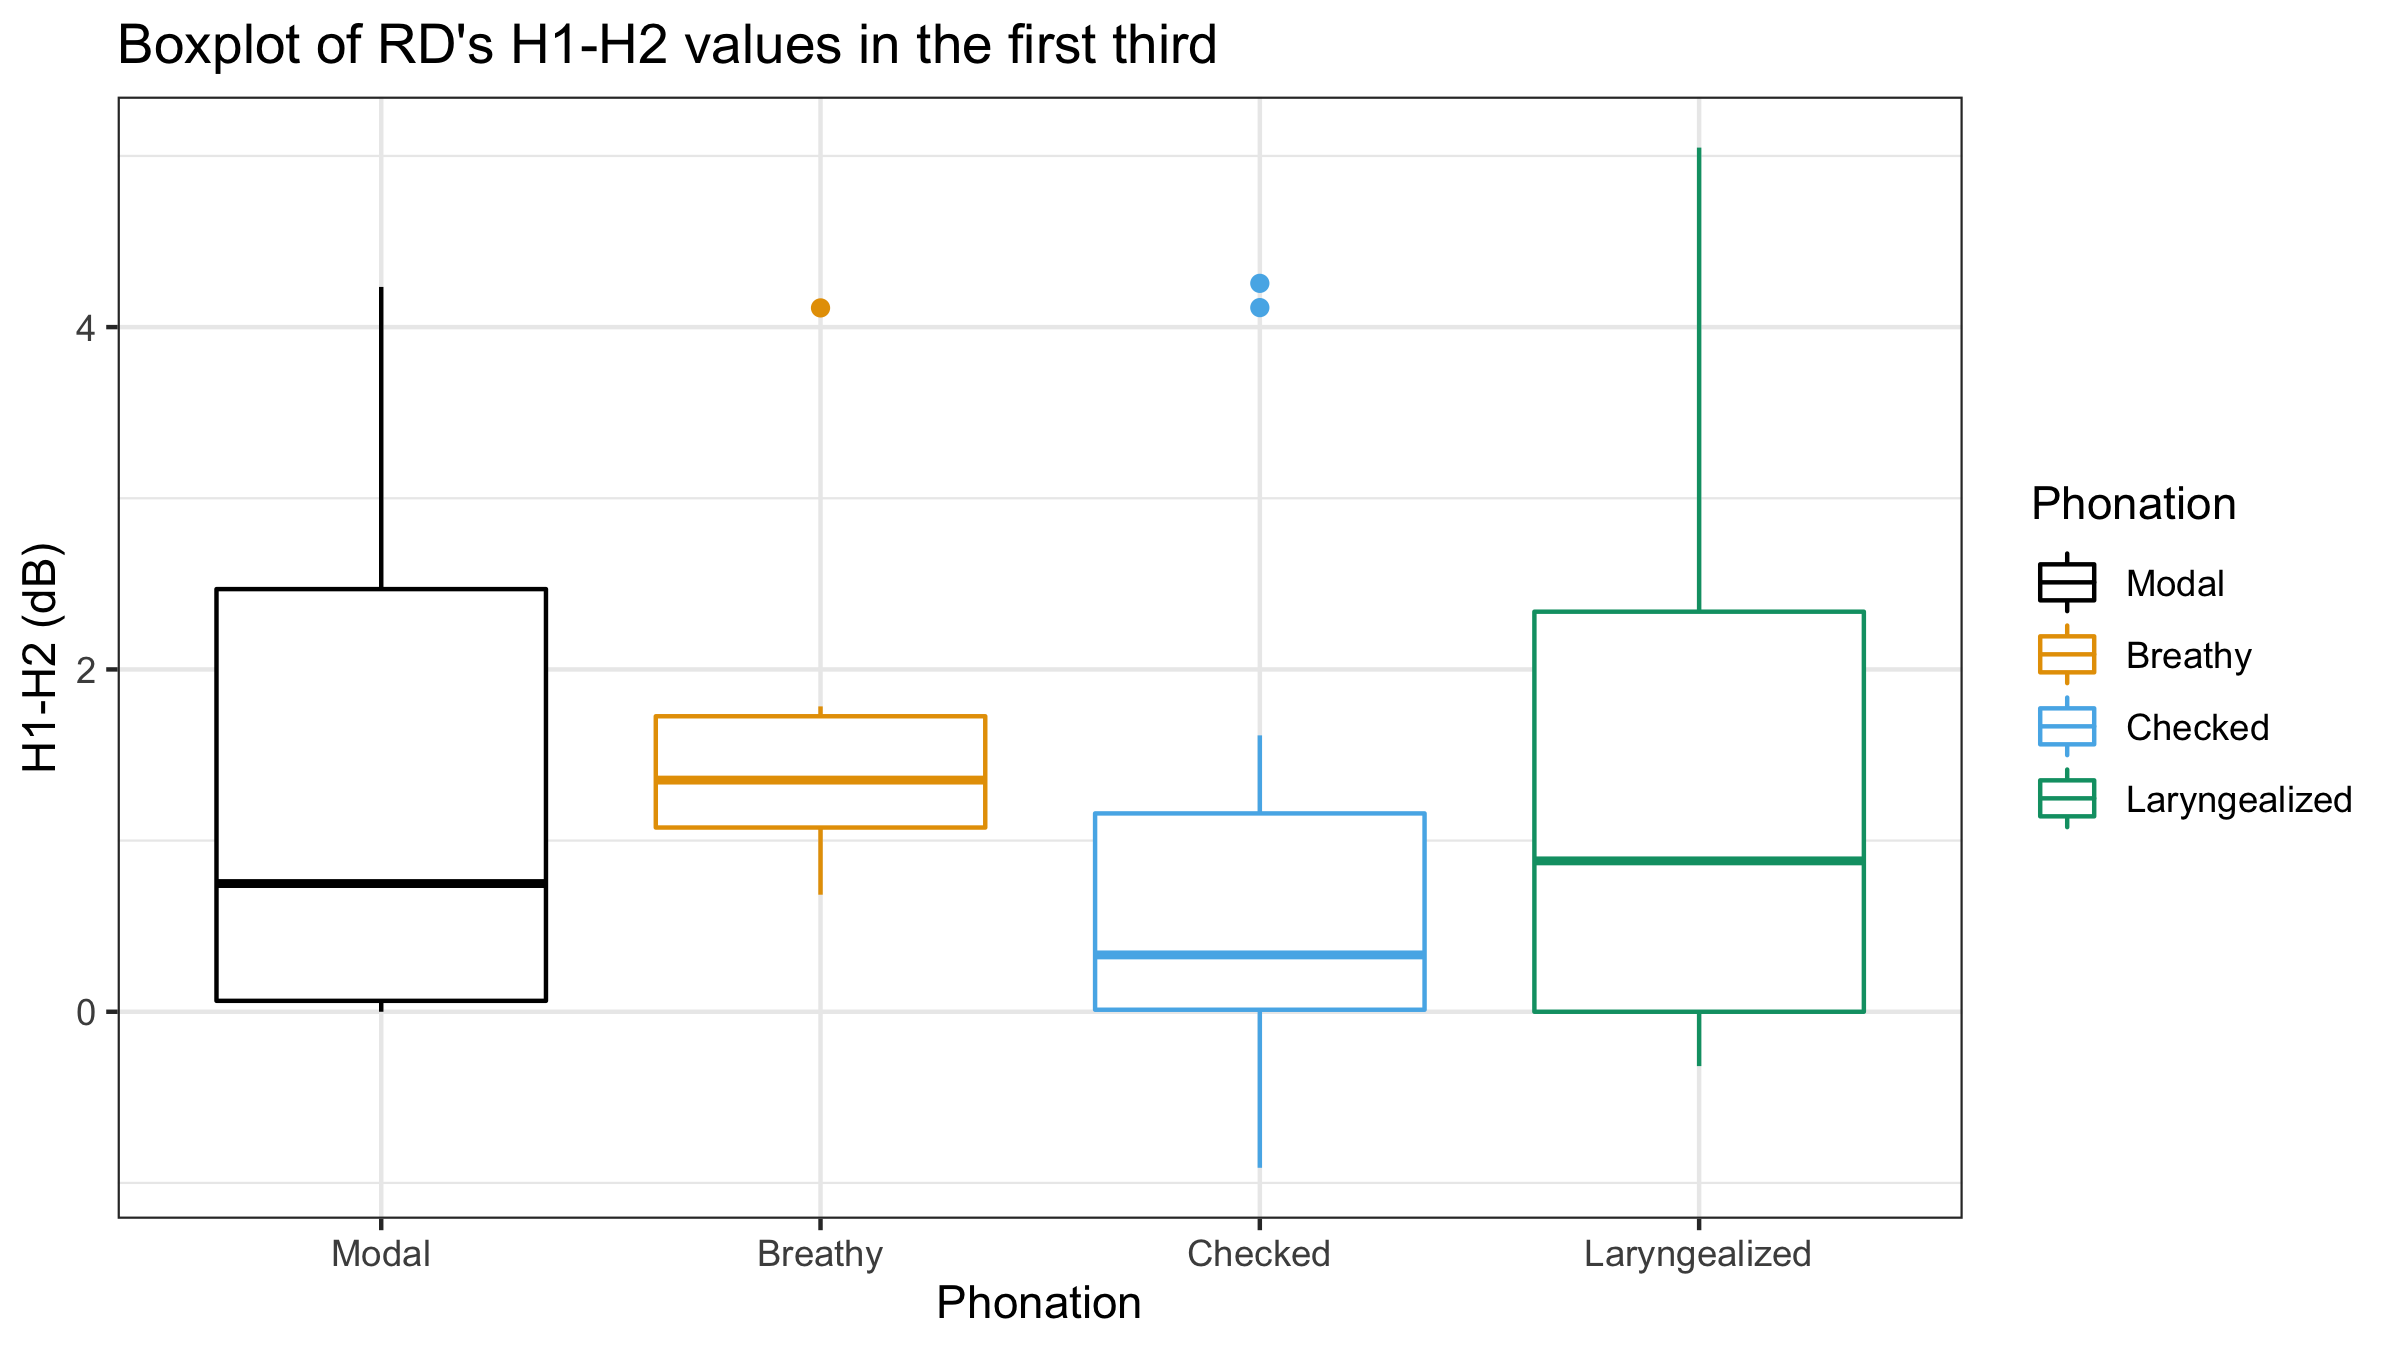
\includegraphics[width=0.9\textwidth]{../mean_RD_h1h2_1st.png}
		\caption{RD's H1-H2 values.}
		\label{fig:RDh1h2first} 
	\end{subfigure}
	\caption{Mean H1-H2 values for the first third of the vowel according to each phonation type. }
	\label{fig:h1h2first}
\end{figure}

\begin{figure}[!ht]
	\centering
	\begin{subfigure}{.5\textwidth}
		\centering
		\includegraphics[width=0.9\textwidth]{../mean_FSR_h1h2_2nd.png}
		\caption{FSR's H1-H2 values.}
		\label{fig:FSRh1h2second} 
	\end{subfigure}%
	\begin{subfigure}{.5\textwidth}
		\centering
		\includegraphics[width=0.9\textwidth]{../mean_RD_h1h2_2nd.png}
		\caption{RD's H1-H2 values.}
		\label{fig:RDh1h2second} 
	\end{subfigure}
	\caption{Mean H1-H2 values for the second third of the vowel according to each phonation type.}
	\label{fig:h1h2second}
\end{figure}

\begin{figure}[!ht]
	\centering
	\begin{subfigure}{.5\textwidth}
		\centering
		\includegraphics[width=0.9\textwidth]{../mean_FSR_h1h2_3rd.png}
		\caption{FSR's H1-H2 values.}
		\label{fig:FSRh1h2third} 
	\end{subfigure}%
	\begin{subfigure}{.5\textwidth}
		\centering
		\includegraphics[width=0.9\textwidth]{../mean_RD_h1h2_3rd.png}
		\caption{RD's H1-H2 values.}
		\label{fig:RDh1h2third} 
	\end{subfigure}
	\caption{Mean H1-H2 values for the final third of the vowel according to each phonation type. }
	\label{fig:h1h2third}
\end{figure}
%------------------------------------
\subsection{H1-A3 spectral-tilt} \label{sec:H1A3}
%------------------------------------

\begin{figure}[!h]
	\centering
	\begin{subfigure}{.5\textwidth}
		\centering
		\includegraphics[width=0.9\textwidth]{../mean_FSR_h1a3_First.png}
		\caption{FSR's H1-A3 values.}
		\label{fig:FSRh1a3first} 
	\end{subfigure}%
	\begin{subfigure}{.5\textwidth}
		\centering
		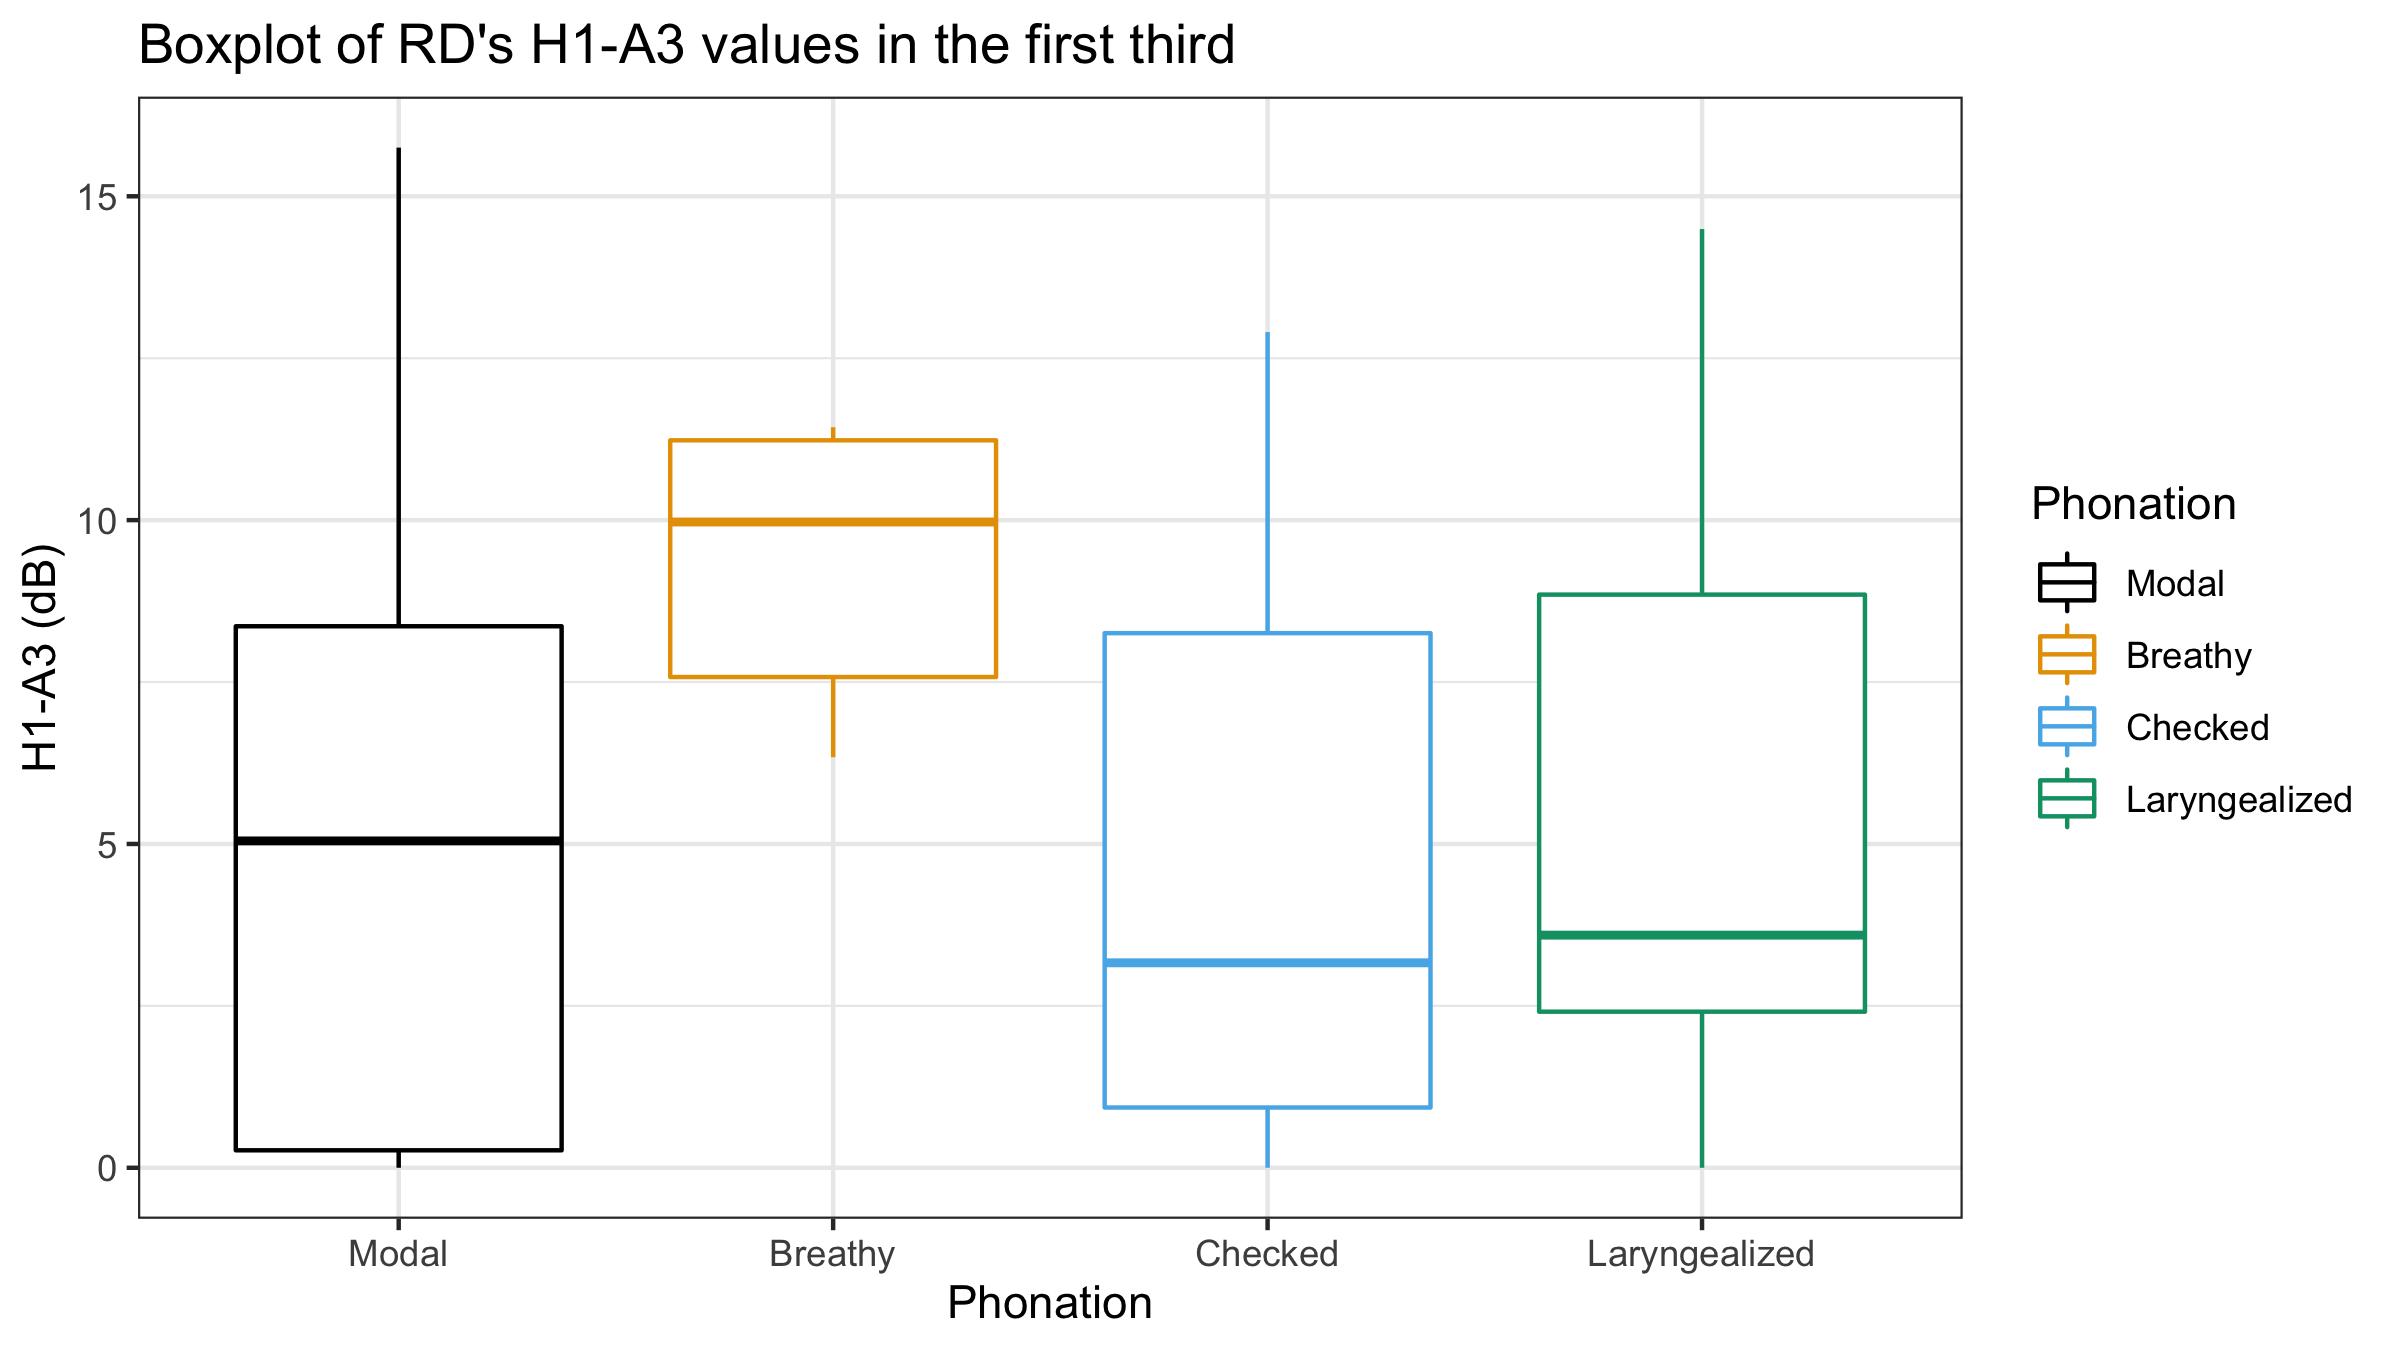
\includegraphics[width=0.9\textwidth]{../mean_RD_h1a3_First.png}
		\caption{RD's H1-A3 values.}
		\label{fig:RDh1a3first} 
	\end{subfigure}
	\caption{H1-A3 values for FSR (a) and RD (b) for the first third of the vowel. }
	\label{fig:h1a3first}
\end{figure}

In the first third of the vowel, RD's mean value for H1-A3 is lower than the modal's H1-A3 value. However, there is a large degree of overlap between modals, checked, and laryngealized H1-A3 values, as evidenced by the boxes covering the same regions, see Figure~\ref{fig:h1a3first}. 

\begin{figure}[!h]
	\centering
	\begin{subfigure}{.5\textwidth}
		\centering
		\includegraphics[width=0.9\textwidth]{../mean_FSR_h1a3_Second.png}
		\caption{FSR's H1-A3 values.}
		\label{fig:FSRh1a3second} 
	\end{subfigure}%
	\begin{subfigure}{.5\textwidth}
		\centering
		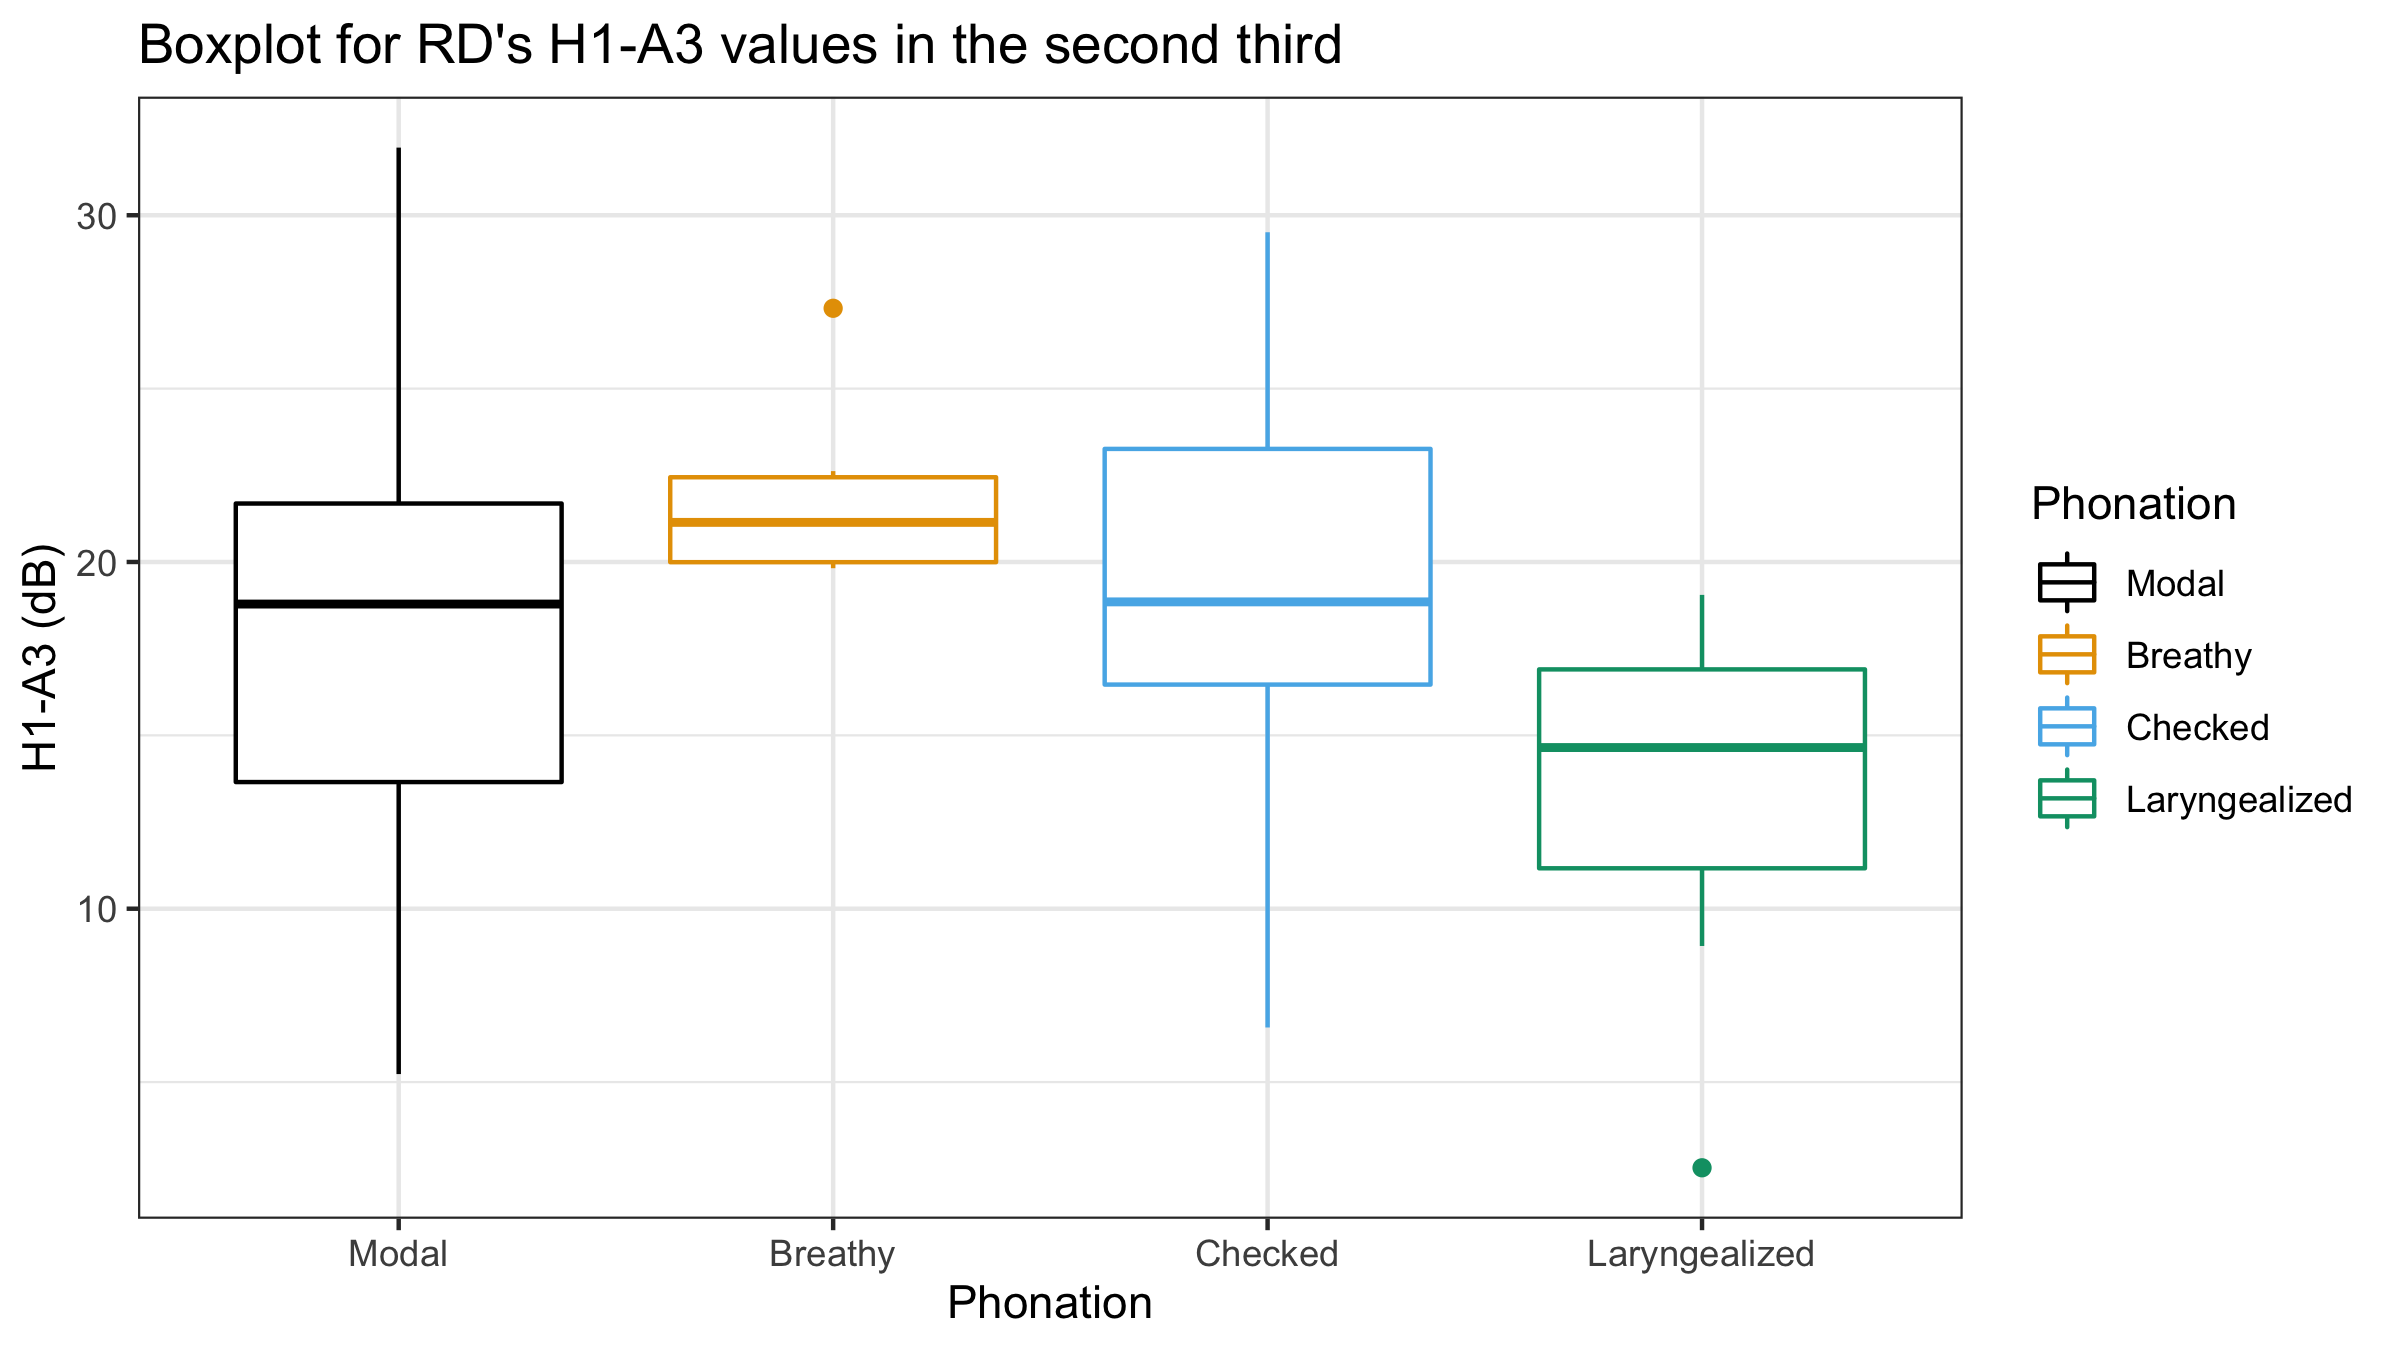
\includegraphics[width=0.9\textwidth]{../mean_RD_h1a3_Second.png}
		\caption{RD's H1-A3' values.}
		\label{fig:RDh1a3second} 
	\end{subfigure}
	\caption{H1-A3 values for FSR (a) and RD (b) for the second third of the vowel. }
	\label{fig:h1a3second}
\end{figure}

In the second third of the vowel, Figure~\ref{fig:h1a3second}, the breathy vowel continues to be higher than the modal vowel. The checked and laryngealized vowels H1-A3 values for FSR are uninformative because of the large degree of overlap. For RD, these same measurements show a lower H1-A3 value than the modals which is consistent with creakier productions of vowels. This lower H1-A3 continues throughout the rest of the vowel for laryngealized vowels, see Figure~\ref{fig:RDh1a3third}. This behavior is consistent with the observation that RD performs creaky voice throughout their production of laryngealized vowels. For the checked vowels, the measurements are very similar to those of the modal vowel. 

In looking at the final portion of the vowels, Figure~\ref{fig:h1a3third}, the measurements continue to show similar behavior to the second portion for both FSR and RD. However, one exception is the lower H1-A3 value for FSR's checked vowels, suggesting that FSR produces a period of creakiness in the last portion of the vowel.

\begin{figure}[!ht]
	\centering
	\begin{subfigure}{.5\textwidth}
		\centering
		\includegraphics[width=0.9\textwidth]{../mean_FSR_h1a3_third.png}
		\caption{FSR's H1-A3 values.}
		\label{fig:FSRh1a3third} 
	\end{subfigure}%
	\begin{subfigure}{.5\textwidth}
		\centering
		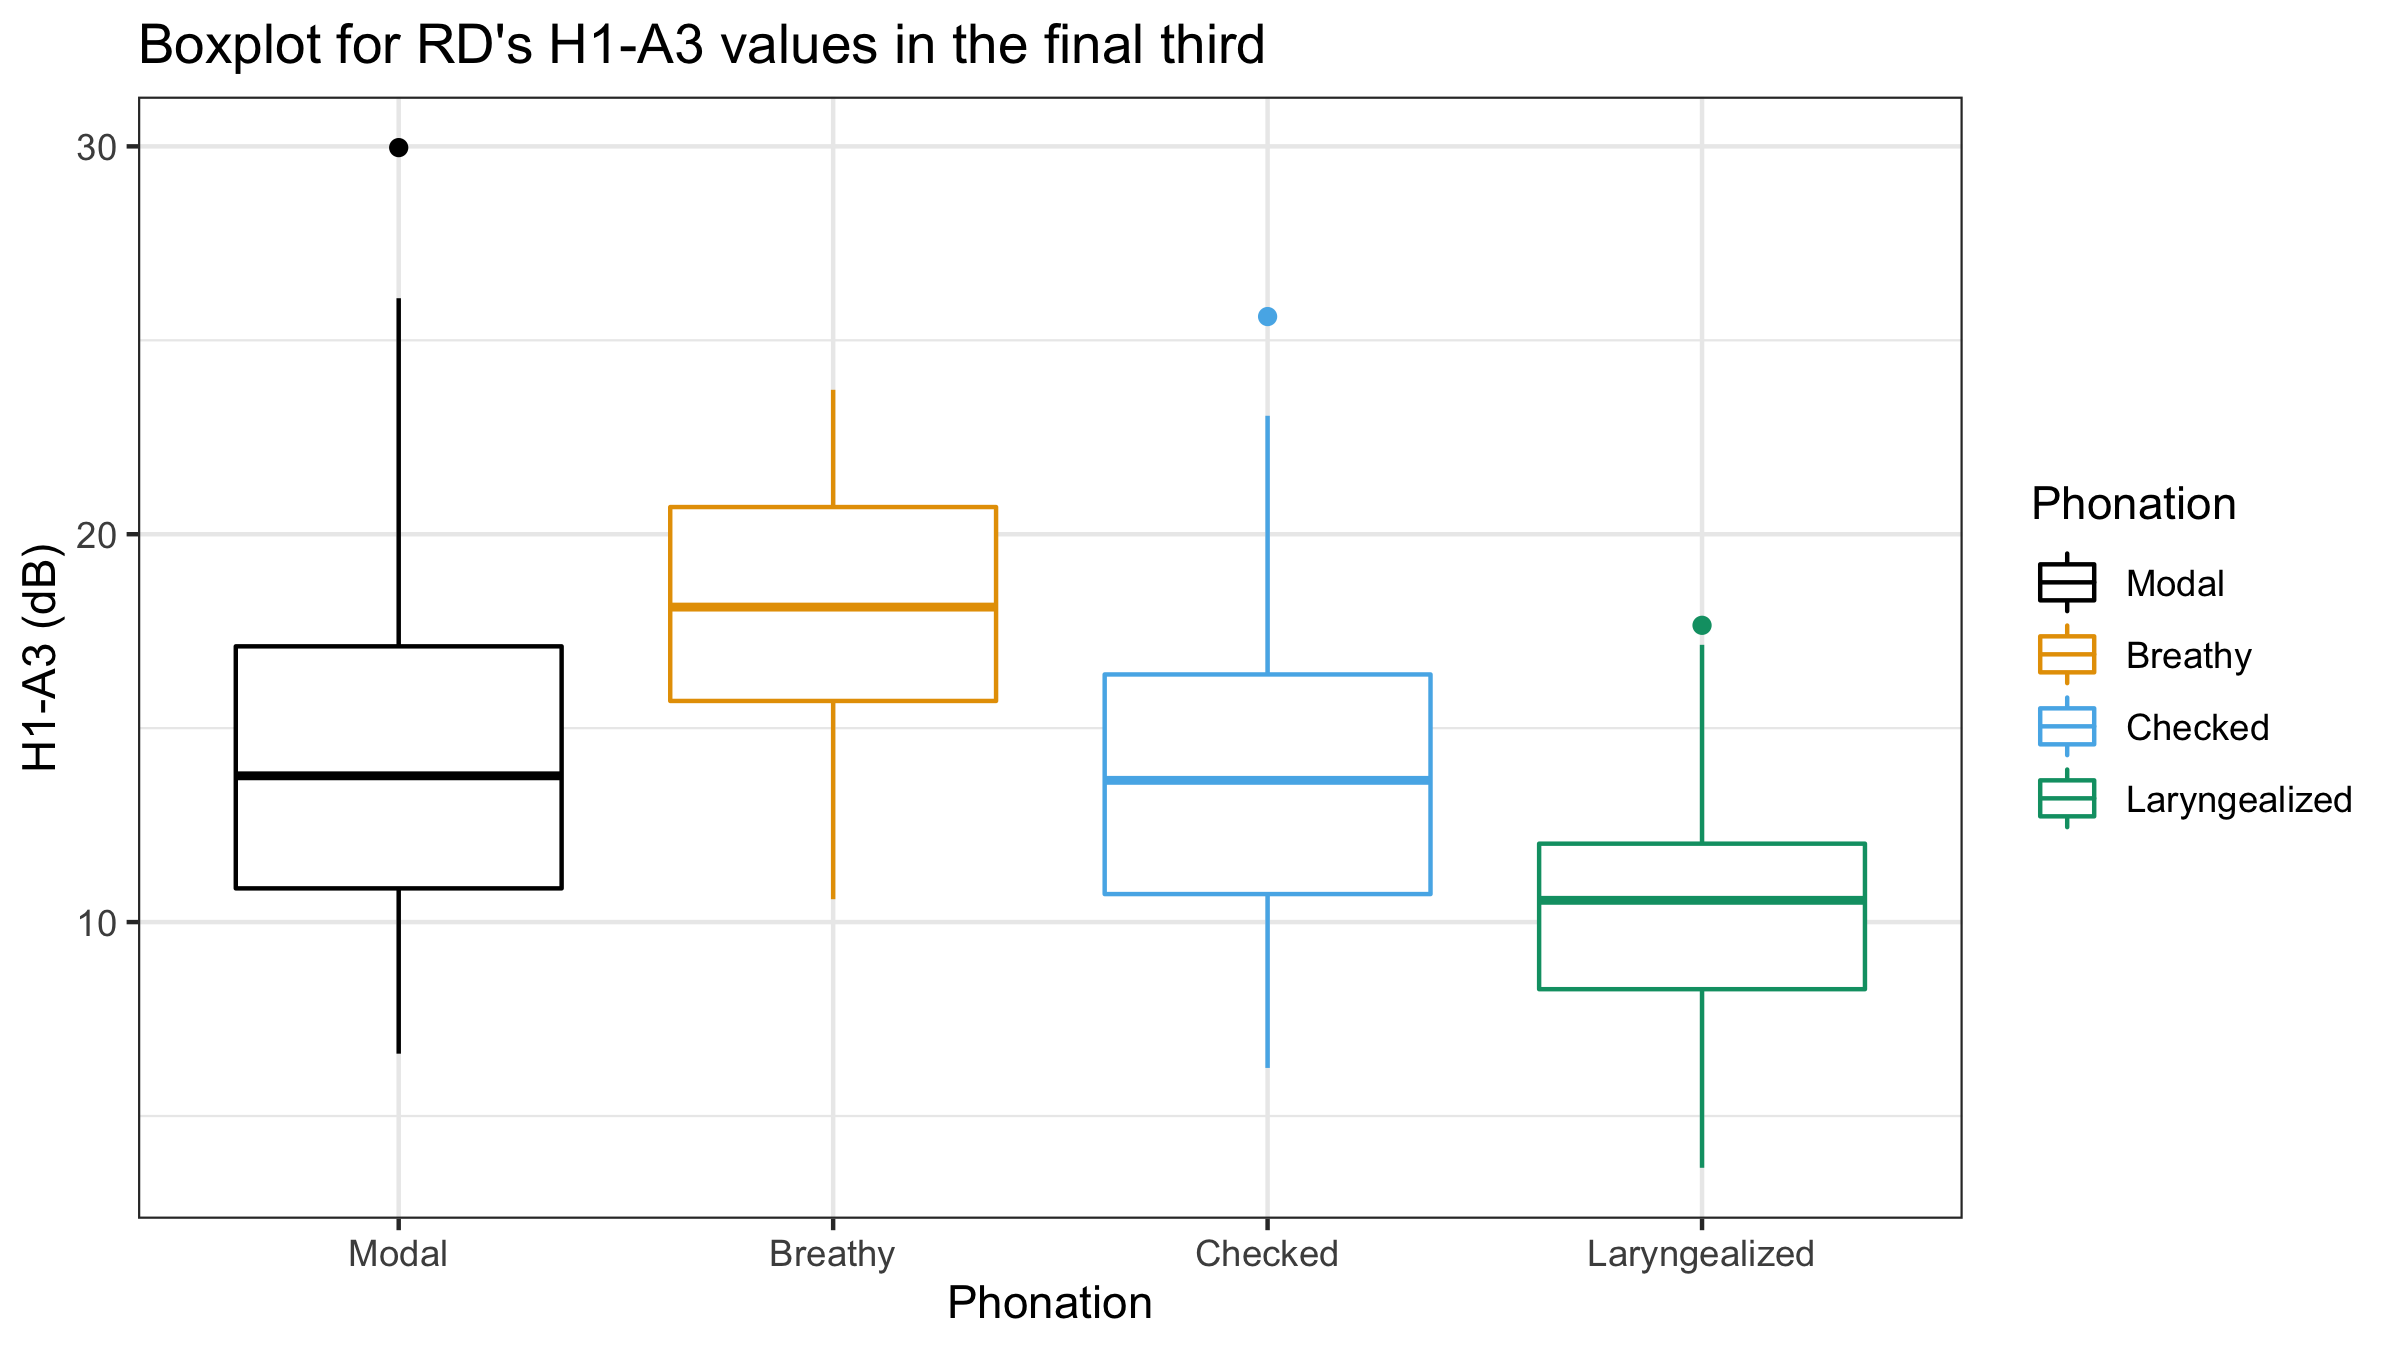
\includegraphics[width=0.9\textwidth]{../mean_RD_h1a3_third.png}
		\caption{RD's H1-A3 values.}
		\label{fig:RDh1a3third} 
	\end{subfigure}
	\caption{H1-A3 values for FSR (a) and RD (b) for the final third of the vowel. }
	\label{fig:h1a3third}
\end{figure}

%------------------------------------
\subsection{Cepstral Peak Prominence} \label{sec:CPP}
%------------------------------------

\begin{figure}[!ht]
	\centering
	\begin{subfigure}{.5\textwidth}
		\centering
		\includegraphics[width=0.9\textwidth]{../mean_FSR_cpp_First.png}
		\caption{FSR's CPP values.}
		\label{fig:FSRcppfirst} 
	\end{subfigure}%
	\begin{subfigure}{.5\textwidth}
		\centering
		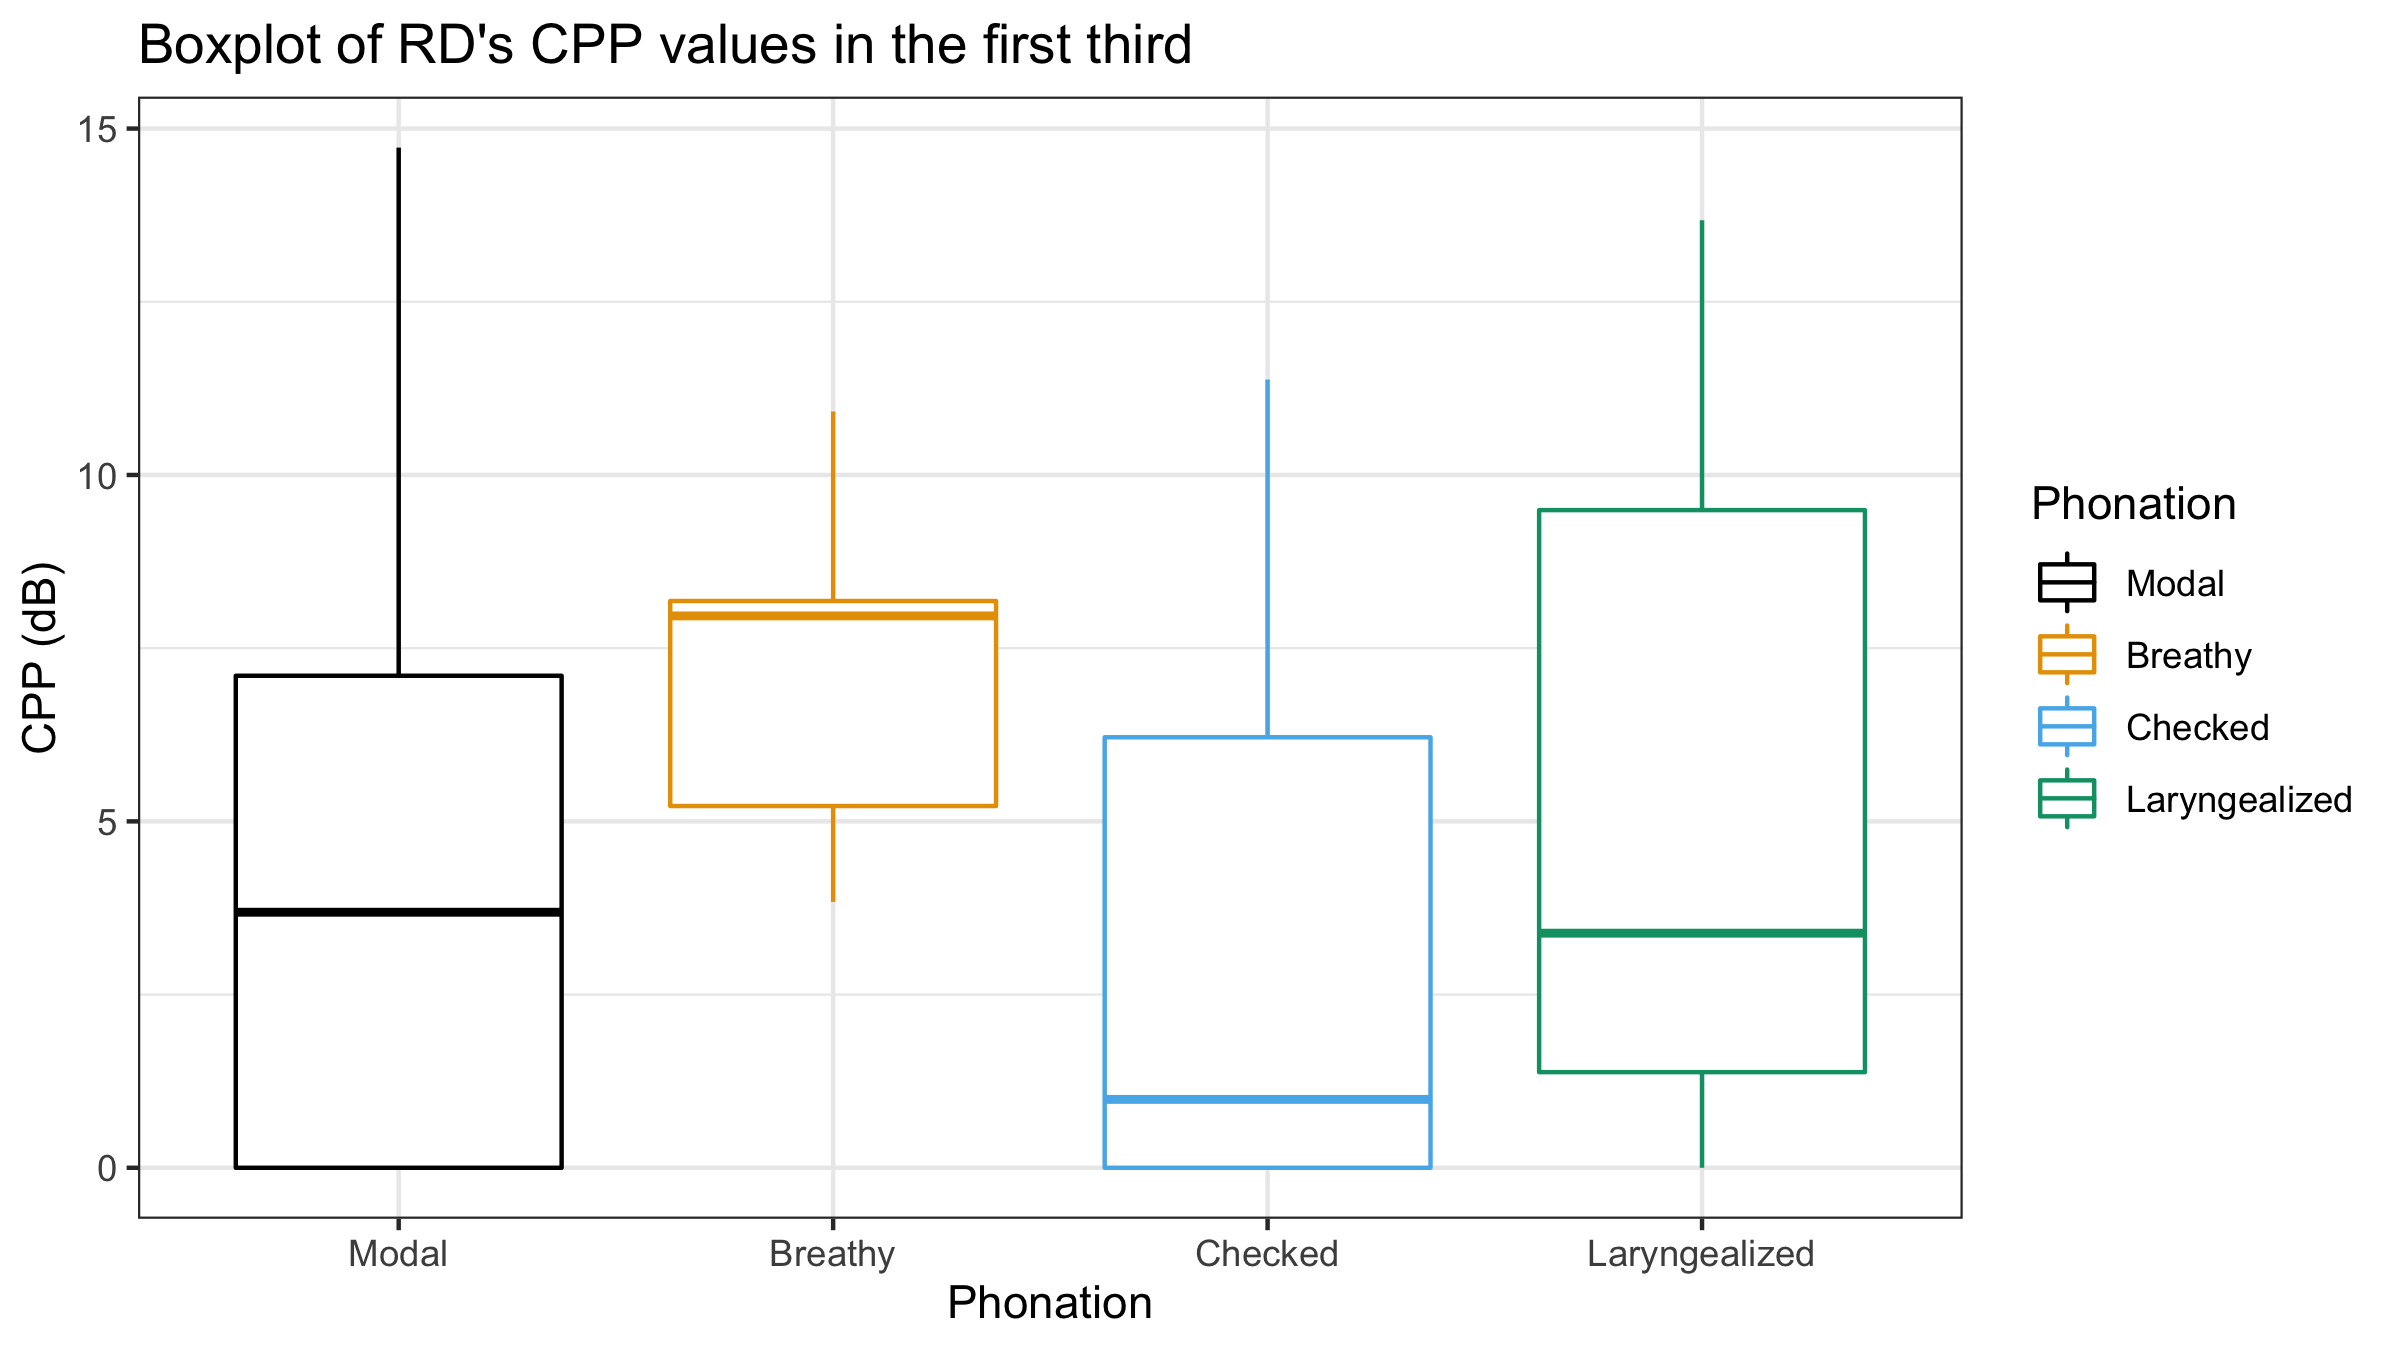
\includegraphics[width=0.9\textwidth]{../mean_RD_cpp_First.png}
		\caption{RD's CPP values.}
		\label{fig:RDcppfirst} 
	\end{subfigure}
	\caption{CPP values for FSR (a) and RD (b) for the first third of the vowel. }
	\label{fig:cppfirst}
\end{figure}

\begin{figure}[!ht]
	\centering
	\begin{subfigure}{.5\textwidth}
		\centering
		\includegraphics[width=0.9\textwidth]{../mean_FSR_cpp_Second.png}
		\caption{FSR's CPP values.}
		\label{fig:FSRcppsecond} 
	\end{subfigure}%
	\begin{subfigure}{.5\textwidth}
		\centering
		\includegraphics[width=0.9\textwidth]{../mean_RD_cpp_Second.png}
		\caption{RD's CPP values.}
		\label{fig:RDcppsecond} 
	\end{subfigure}
	\caption{CPP values for FSR (a) and RD (b) for the second third of the vowel. }
	\label{fig:cppsecond}
\end{figure}

\begin{figure}[!ht]
	\centering
	\begin{subfigure}{.5\textwidth}
		\centering
		\includegraphics[width=0.9\textwidth]{../mean_FSR_cpp_third.png}
		\caption{FSR's CPP values.}
		\label{fig:FSRcppthird} 
	\end{subfigure}%
	\begin{subfigure}{.5\textwidth}
		\centering
		\includegraphics[width=0.9\textwidth]{../mean_RD_cpp_third.png}
		\caption{RD's CPP values.}
		\label{fig:RDcppthird} 
	\end{subfigure}
	\caption{CPP values for FSR (a) and RD (b) for the final third of the vowel. }
	\label{fig:cppthird}
\end{figure}

%------------------------------------
\subsection{Statistical results} \label{sec:Stats}
%------------------------------------

\begin{table}[!h]
	\centering
	\caption{Results of the mixed-effects linear regression analysis on the first third of the vowel for H1-H2. }
	\label{tab:H1H2_First}
	 \begin{tabular}{llllll}
	  \lsptoprule
						&  Estimate  & Std. Error & df & t value & p-value \\
	  	Breathy   		&  -0.3049  &   0.5795 & 116.4255 &  -0.526  &  0.600 \\
		Checked    		&  -0.4731  &   0.4029 & 145.6184 &  -1.174  &  0.242 \\
		Laryngealized	&  -0.2938  &   0.4675 & 101.9977 &  -0.629  &  0.531 \\
	  \lspbottomrule
	 \end{tabular}
\end{table}

As can be recalled from Section~\ref{sec:H1H2}, both FSR and RD show a lower value for H1-H2 for breathy vowels in the last two-thirds of the vowels when compared to the model vowel's H1-H2 values. The results of the statistical analysis for the last two-thirds of the vowel, presented in Table~\ref{tab:H1H2_Second} and Table~\ref{tab:H1H2_Third}, show that this behavior is significant.

At no point do the other phonation types reach significance with respect to H1-H2. 

\begin{table}[!h]
	\centering
	\caption{Results of the mixed-effects linear regression analysis on the second third of the vowel for H1-H2. }
	\label{tab:H1H2_Second}
	 \begin{tabular}{llllll}
	  \lsptoprule
						&  Estimate  & Std. Error & df & t value & p-value \\
	  	Breathy   		&  -3.4158  &   1.3400 & 126.9590 &  -2.549  &  0.0120 \\
		Checked    		&  -1.7466  &   0.9197 & 146.9995 &  -1.899  &  0.0595 \\
		Laryngealized	&  -0.7405  &   1.0852 & 117.0669 &  -0.682  &  0.4963 \\
	  \lspbottomrule
	 \end{tabular}
\end{table}

\begin{table}[!h]
	\centering
	\caption{Results of the mixed-effects linear regression analysis on the final third of the vowel for H1-H2. }
	\label{tab:H1H2_Third}
	 \begin{tabular}{llllll}
	  \lsptoprule
						&  Estimate  & Std. Error & df & t value & p-value \\
	  	Breathy   		&  -2.2131  &   1.0291 & 125.2092 &  -2.151  &  0.0334 \\
		Checked    		&  -1.3487  &   0.6952 & 146.2461 &  -1.940  &  0.0543 \\
		Laryngealized	&  -0.8676  &   0.8202 & 116.8963 &  -1.058  &  0.2923 \\
	  \lspbottomrule
	 \end{tabular}
\end{table}

The second statistical analysis for the H1-A3 measurement shows some very clear behavior for breathy voice. As can be recalled from Section~\ref{sec:H1A3}, we observe that breathy voice is clearly identified in all portions of the vowel with an elevated H1-A3 value when compared to the model vowels' values. We see that at all portions of the vowel, as seen in Tables~\ref{tab:H1A3_First}, \ref{tab:H1A3_Second}, \ref{tab:H1A3_Third} show significance.  

\begin{table}[!h]
	\centering
	\caption{Results of the mixed-effects linear regression analysis on the first third of the vowel for H1-A3. }
	\label{tab:H1A3_First}
	 \begin{tabular}{llllll}
	  \lsptoprule
						&  Estimate  & Std. Error & df & t value & p-value \\
	  	Breathy   		&  4.29036  &  1.31288 & 137.12067 &  3.268  &  0.00137\\
		Checked    		&  0.15001  &  0.84476 & 134.62215 &  0.178  &  0.85932 \\
		Laryngealized	& -0.05694  &  1.07130 & 137.16596 & -0.053  &  0.95769\\
	  \lspbottomrule
	 \end{tabular}
\end{table}

\begin{table}[!h]
	\centering
	\caption{Results of the mixed-effects linear regression analysis on the second third of the vowel for H1-A3. }
	\label{tab:H1A3_Second}
	 \begin{tabular}{llllll}
	  \lsptoprule
						&  Estimate  & Std. Error & df & t value & p-value \\
	  	Breathy   		&  4.398    &  2.027 & 147.003 &  2.169 &  0.0317 \\
		Checked    		&  1.195    &  1.426 & 147.000 &  0.838 &  0.4033  \\
		Laryngealized	& -2.694    &  1.627 & 147.001 & -1.656 &  0.0998 \\
	  \lspbottomrule
	 \end{tabular}
\end{table}

\begin{table}[!h]
	\centering
	\caption{Results of the mixed-effects linear regression analysis on the final third of the vowel for H1-A3. }
	\label{tab:H1A3_Third}
	 \begin{tabular}{llllll}
	  \lsptoprule
						&  Estimate  & Std. Error & df & t value & p-value \\
	  	Breathy   		&  5.2928   &  1.7966 & 127.0400 &  2.946 & 0.00383 \\
		Checked    		& -0.7825   &  1.2487 & 147.1011 & -0.627 & 0.53189 \\
		Laryngealized	& 0.2669    &  1.4224 & 117.4917 &  0.188 & 0.85151 \\
	  \lspbottomrule
	 \end{tabular}
\end{table}

However, the other phonations failed to reach significance when evaluated against H1-A3.

It is important to realize that at this point that H1-H2 and H1-A3 both have failed to account for checked and laryngealized phonations. This is also born out by the observations in Sections~\ref{sec:H1H2} and \ref{sec:H1A3} which did not show any remarkable differences from the model. When we consider CPP we see both checked and laryngealized vowels clearly differentiated. This is born out in the statistical analysis. This analysis took CPP as fixed and speaker and word as random. This analysis showed that the first third of the vowel, Table~\ref{tab:CPP_First} both breathy and checked voice were identifiable with CPP. 

% Based on the results of the statistical analysis, CPP is informative for differentiating checked from laryngealized voice. Laryngealized voice shows a statistically significance in the second-third of the vowel. This is consistent with the observed behavior approximately in the center of the vowel. Despite the differences in how the the laryngealized vowels are produced between the speakers, there is a difference in the CPP value in the middle of the vowel it 

\begin{table}[!h]
	\centering
	\caption{Results of the mixed-effects linear regression analysis on the first third of the vowel for CPP. }
	\label{tab:CPP_First}
	 \begin{tabular}{llllll}
	  \lsptoprule
						&  Estimate  & Std. Error & df & t value & p-value \\
	  	Breathy   		&  3.4470   &  1.1743 & 145.9760 &  2.935 & 0.00387 \\
		Checked    		& -1.4190   &  0.7088 & 120.5020 & -2.002 & 0.04754 \\
		Laryngealized	&  0.8240   &  0.9530 & 147.0083 &  0.865 & 0.38868 \\
	  \lspbottomrule
	 \end{tabular}
\end{table}

When considering the second-third of the vowel, Table~\ref{tab:CPP_Second}, laryngealized vowels become clearly identifiable by CPP which is born out by the significance of laryngealized phonation and the lack of significance with breathy and checked. This is consistent with the observation that somewhere in the middle of the vowel there is either a full glottal stop or a period of creakiness in the two speakers that were evaluated for this study. This observation also bears witness to observations made by \citet{avelinoAcousticElectroglottographicAnalyses2010} about the how each of the different manners that laryngealized vowels are produced in Yalálag Zapotec each have a period of model phonation followed by a aperiodicity or a glottal constriction beginning in the middle of the vowel. 

\begin{table}[!h]
	\centering
	\caption{Results of the mixed-effects linear regression analysis on the second third of the vowel for CPP. }
	\label{tab:CPP_Second}
	 \begin{tabular}{llllll}
	  \lsptoprule
						&  Estimate  & Std. Error & df & t value & p-value \\
	  	Breathy   		&  1.5044   &  1.4073 & 128.0083 &  1.069 & 0.287094 \\
		Checked    		& -0.5804   &  0.9789 & 146.0792 & -0.593 & 0.554154 \\
		Laryngealized	& -2.2898   &  1.1354 & 117.6213 & -2.017 & 0.046006 \\
	  \lspbottomrule
	 \end{tabular}
\end{table}

In considering the final portion of the vowel, Table~\ref{tab:CPP_Third}, the statistical analysis shows that only checked vowels can be reliably determined using CPP. This observations is consistent with the facts that checked phonation consists of a period of creakiness or full glottal closure at the end of the vowel. The other phonation types fail to reach significance.

\begin{table}[!h]
	\centering
	\caption{Results of the mixed-effects linear regression analysis on the final third of the vowel for CPP. }
	\label{tab:CPP_Third}
	 \begin{tabular}{llllll}
	  \lsptoprule
						&  Estimate  & Std. Error & df & t value & p-value \\
	  	Breathy   		&  1.6391   &  1.0173  & 139.8563 &  1.611 & 0.10939 \\
		Checked    		& -2.1386   &  0.6449  & 129.1392 & -3.316 & 0.00119 \\
		Laryngealized	& -1.1158   &  0.8142  & 140.5570 & -1.370 & 0.17274\\
	  \lspbottomrule
	 \end{tabular}
\end{table}

%------------------------------------
\section{Discussion} \label{sec:Discussion}
%------------------------------------

%------------------------------------
\subsection{Laryngeal Complexity Hypothesis} \label{sec:LCH}
%------------------------------------

\begin{itemize}
	\item The Laryngeal Complexity Hypothesis (LCH) has its origin in work from \citet{silvermanLaryngealComplexityOtomanguean1997,blankenshipTimeCourseBreathiness1997,blankenshipTimingNonmodalPhonation2002}.
	\item The LCH claims that languages that have both tone and phonation need them to be phased/ordered with respect to each other. 
	\item This is required because it is assumed that the same mechanism for tone is also responsible for phonation. 
	\begin{itemize}
		\item Tone is the rate of vocal fold vibration. 
		\item \citet{ladefogedPreliminariesLinguisticPhonetics1971,gordonPhonationTypesCrosslinguistic2001} argued that phonation exists on a single dimension ranging from opened vocal folds to closed vocal folds. 
	\end{itemize} 
	\item The variation in how open or closed the vocal folds are correspond to whether or not the sound produced is breathy or creaky. 
	\item \citet{ladefogedPreliminariesLinguisticPhonetics1971,gordonPhonationTypesCrosslinguistic2001} summarized this assumption in the diagram found in Figure~\ref{fig:Phonation}.
\end{itemize}
\begin{figure}[!h]
	\centering
	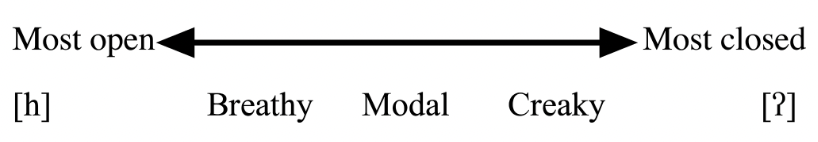
\includegraphics[width=.6\textwidth]{../Phonation.png}
	\caption{Simplified one-deminsional model for phonation. Based on \citet{ladefogedPreliminariesLinguisticPhonetics1971,gordonPhonationTypesCrosslinguistic2001}}.
	\label{fig:Phonation}
\end{figure}
\vspace{-2ex}
\begin{itemize}
	\item Because the same organ is responsible for these two different phenomena there is a mismatch in trying to produce both at the same time. 
	\item The LCH assumes that there needs to be a strict ordering in the glottal gestures. 
	\item If the gestures were overlapped there will be a perturbation of the tone and the listeners will not be able to reliably differentiate what the tone is.
	\item The LCH assumes that there is a close link between production and perception. 
	\item This assumption places the responsibility on making sure the acoustic cues are the most perceptually salient on the speaker. 
	\item In Figure~\ref{fig:GlottalGestures}, which is taken from \citet{dicanioCoarticulationToneGlottal2012}, the cue for tone is represented by the Pitch Target and the Glottal Gesture represents the gestures needed to produce phonation. 
\end{itemize}
	\begin{figure}[!ht]
		\centering
		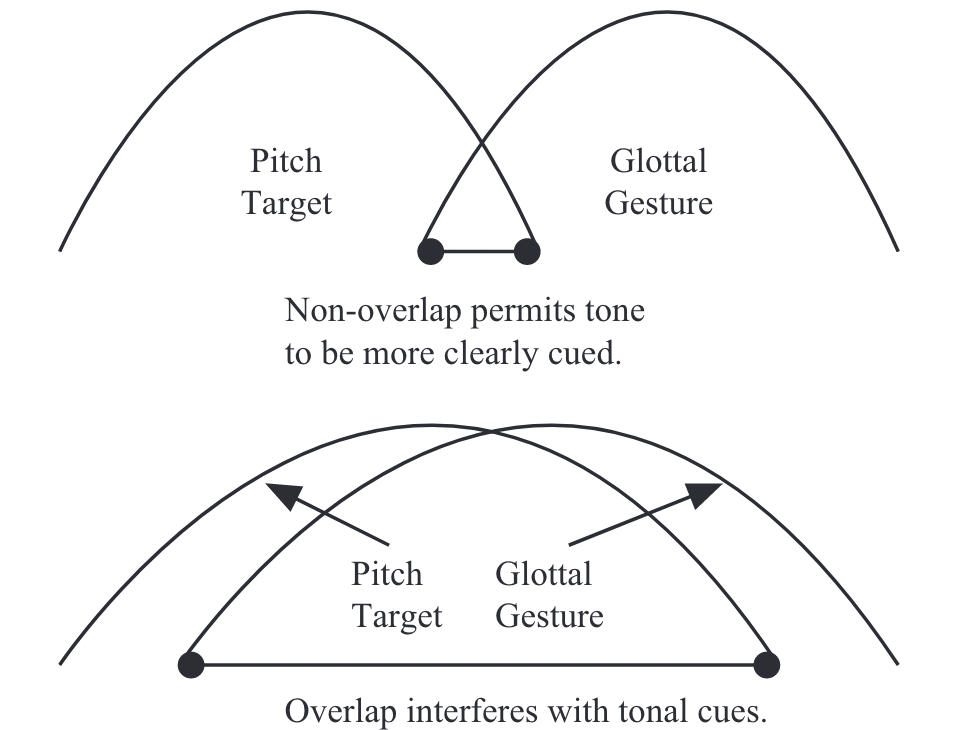
\includegraphics[width=.5\textwidth]{../Gestures.png}
		\caption{Representation taken from \citet{dicanioCoarticulationToneGlottal2012}.}
		\label{fig:GlottalGestures}
	\end{figure}
\begin{itemize}
	\item \citet{dicanioCoarticulationToneGlottal2012} found that when the magnitude of coarticulation for glottal consonants occurs on the vowels there is a strong correlation between the magnitude of overlap and the amount of perturbation in the f0 signal. If, however, the degree of overlap was minor then the acoustic signal had little to no perturbation.
	\item Jalapa Mazatec is a language with both contrastive tone and phonation and \citet{garellekAcousticConsequencesPhonation2011} validated the claims made by the LCH, in that tone and phonation seemed to be ordered with each other when it comes to at least one of the phonation types.
\end{itemize}

%------------------------------------
\subsection{Laryngeal Articulator Model} \label{sec:LAM}
%------------------------------------

\begin{table}[!ht]
	\centering
	\caption{A list of the different nodes and their abbreviations in the Laryngeal Articulator Model.}
	\label{tab:States}
	 \begin{tabular}{ll}
	  \lsptoprule
	  States/Nodes	&	 Physiological description \\
	  \hline
	  	vfo   	&  vocal folds open (abducted) \\
		vfc    	&  vocal folds closed (adducted/prephonation)\\
		epc   	&  epilaryngeal constriction\\
		epv			&  epilaryngeal vibration \\
		tfr 		&  tongue fronting \\
		tre 		&  tongue retraction \\
		tra 		&  tongue raising \\
		tdb 		&	 tongue double bunching\\
		↑lx     &  raised larynx\\
		↓lx			&  lowered larynx\\
		Hf0			&  increased vocal fold tension, less vibrating mass (high f0)\\
		Lf0			&  decreased vocal fold tension, more vibrating mass (lower f0)\\
	  \lspbottomrule
	 \end{tabular}
\end{table}

These twelve nodes not only represent the interactions of the larynx but also represents actual physiological representations. This means that any given node represents what is occurring with a given part of the larynx. For example, the node `epc'  represents any epilaryngeal constriction when activated. Now these nodes are not just independent entities but interact in complex ways with other nodes. These interactions are best captured as a network or web of nodes as seen in Figure~\ref{fig:LAMNetwork}. 

\begin{figure}[!ht]
	\centering
	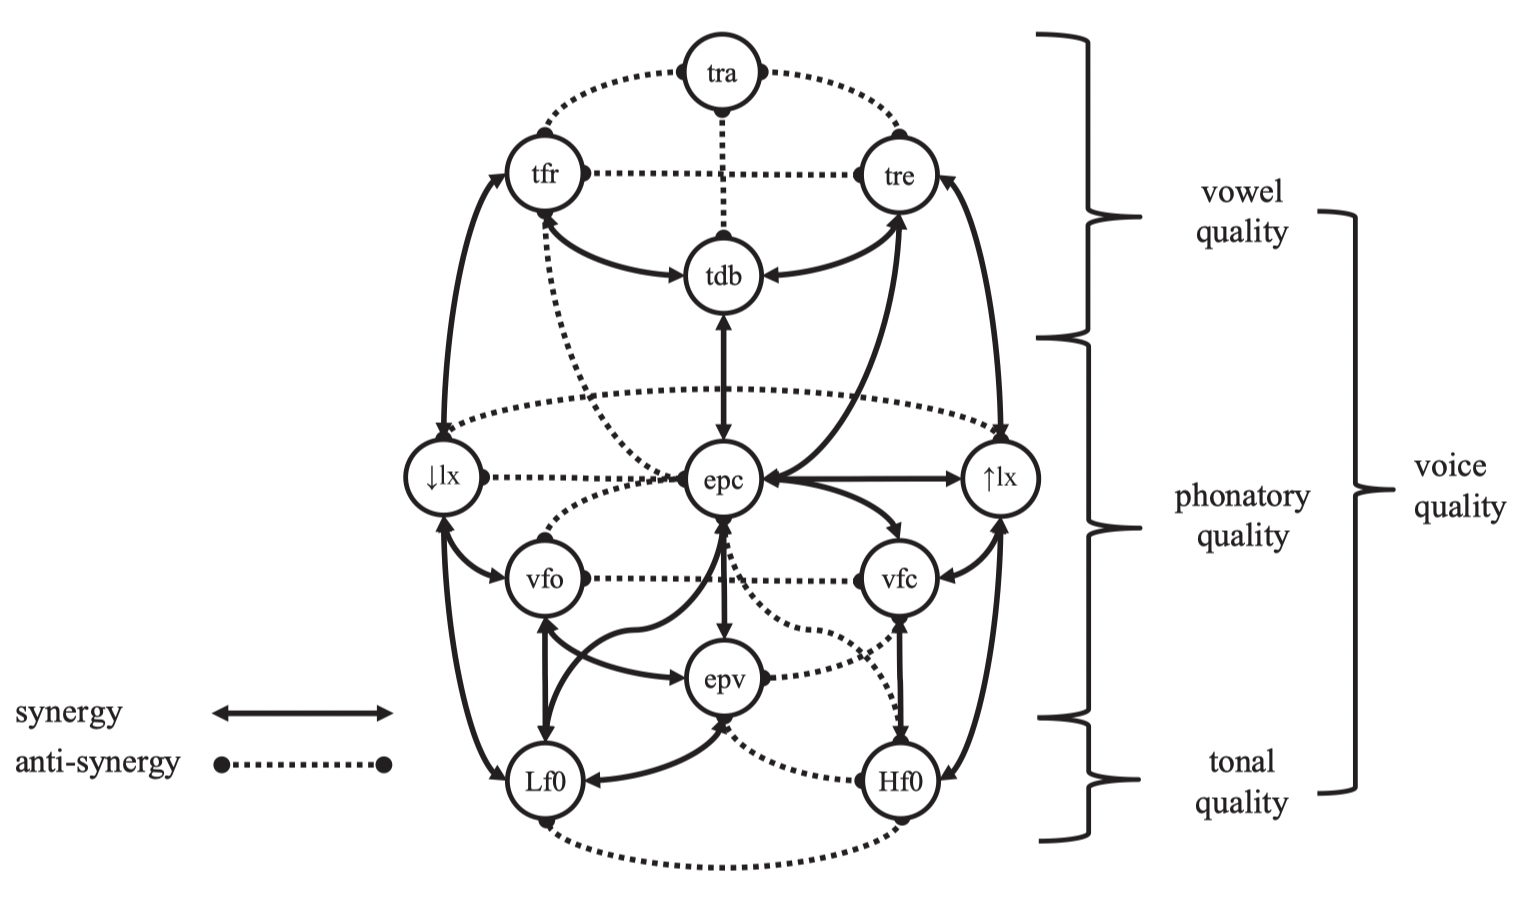
\includegraphics[width=0.9\textwidth]{../LAMNetwork.png}
	\caption{Network of synergistic and anti-synergistic nodes in the Laryngeal Articulator Model. Taken from \citet{eslingVoiceQualityLaryngeal2019}.}
	\label{fig:LAMNetwork}
\end{figure}

%------------------------------------
\section{Conclusion} \label{sec:Conclusion}
%------------------------------------

%------------------------------------
%\subsection{} \label{}
%------------------------------------

%------------------------------------
%BIBLIOGRAPHY
%------------------------------------

%\singlespacing
% \nocite{*}
\printbibliography[heading=bibintoc]

\end{document} 